\documentclass{article}
\usepackage[utf8]{inputenc}
\usepackage[T1]{fontenc}
\usepackage[french]{babel}

% ------------------------- Color table ----------------------------------------
\usepackage{multirow}
\usepackage[table]{xcolor}
\definecolor{maroon}{cmyk}{0,0.87,0.68,0.32}
% ------------------------------------------------------------------------------

\usepackage{amscd}
\usepackage{amsthm}
\usepackage{physics}
\usepackage[left=2.2cm,right=2.2cm,top=2cm,bottom=2cm]{geometry}
\usepackage{textcomp,gensymb} %pour le °C, et textcomp pour éviter les warning
\usepackage{graphicx} %pour les images
\usepackage{caption}
\usepackage{subcaption}
\usepackage[colorlinks=true,
	breaklinks=true,
	citecolor=blue,
	linkcolor=blue,
	urlcolor=blue]{hyperref} % pour insérer des liens
\usepackage{epstopdf} %converting to PDF
\usepackage[export]{adjustbox} %for large figures

\usepackage{array}
\usepackage{dsfont}% indicatrice : \mathds{1}


% -------------------------- Mathematics ---------------------------------------
\graphicspath{{images/}{../images/}} % For the images path
% ------------------------------------------------------------------------------

% -------------------------- Mathematics ---------------------------------------
\usepackage{mathrsfs, amsmath, amsfonts, amssymb}
\usepackage{bm}
\usepackage{mathtools}
\usepackage[Symbol]{upgreek} % For pi \uppi different from /pi
\newcommand{\R}{\mathbb{R}} % For Real space

% ------------------------------------------------------------------------------


% -------------------------- Code format ---------------------------------------
\usepackage[numbered,framed]{matlab-prettifier}
\lstset{
	style              = Matlab-editor,
	basicstyle         = \mlttfamily,
	escapechar         = '',
	mlshowsectionrules = true,
}
% ------------------------------------------------------------------------------

% ------------------------- Blbiographie --------------------------------------
\usepackage[backend=biber, style=ieee]{biblatex}
\addbibresource{biblio.bib}
% ------------------------------------------------------------------------------


\setcounter{tocdepth}{4} %Count paragraph
\setcounter{secnumdepth}{4} %Count paragraph
\usepackage{float}

\usepackage{graphicx} % for graphicspath
% \graphicspath{{../images/}}

\usepackage{array,tabularx}
\newcolumntype{L}[1]{>{\raggedright\let\newline\\\arraybackslash\hspace{0pt}}m{#1}}
\newcolumntype{C}[1]{>{\centering\let\newline\\\arraybackslash\hspace{0pt}}m{#1}}
\newcolumntype{R}[1]{>{\raggedleft\let\newline\\\arraybackslash\hspace{0pt}}m{#1}}

% to start counting section to 6


%%%%%%%%%%%%%%%%%%%%%%%%%%%%%%%%%%%%%%%%%%%
% Header
%%%%%%%%%%%%%%%%%%%%%%%%%%%%%%%%%%%%%%%%%%%

\renewcommand{\assignmenttitle}{Assignment 2 :Image classification}
\renewcommand{\studentname}{Vincent Matthys}
\renewcommand{\email}{vincent.matthys@ens-paris-saclay.fr}

% renew (sub)section to get alpanumeric characters
\renewcommand{\thesection}{\Alph{section}}

%%%%%%%%%%%%%%%%%%%%%%%%%%%%%%%%%%%%%%%%%%%
% Syntax for using figure macros:
%%%%%%%%%%%%%%%%%%%%%%%%%%%%%%%%%%%%%%%%%%%

% \singlefig{filename}{scalefactor}{caption}{label}
% \doublefig{\subfig{filename}{scalefactor}{subcaption}{sublabel}}
%           {\subfig{filename}{scalefactor}{subcaption}{sublabel}}
%           {global caption}{label}
% \triplefig{\subfig{filename}{scalefactor}{subcaption}{sublabel}}
%           {\subfig{filename}{scalefactor}{subcaption}{sublabel}}
%           {\subfig{filename}{scalefactor}{subcaption}{sublabel}}
%           {global caption}{label}
%
% Tips:
% - with scalefactor=1, a single figure will take the whole page width; a double figure, half page width; and a triple figure, a third of the page width
% - image files should be placed in the image folder
% - no need to put image extension to include the image
% - for vector graphics (plots), pdf figures are suggested
% - for images, jpg/png are suggested
% - labels can be left empty {}

%%%%%%%%%%%%%%%%%%%%%%%%%%%%%%%%%%%%%%%%%%%
% Beginning of assignment
%%%%%%%%%%%%%%%%%%%%%%%%%%%%%%%%%%%%%%%%%%%
\begin{document}
\maketitle

\part{Training and testing an Image Classifier}

\section{Data preparation and feature extraction}


\question{QA1: Why is the spatial tiling used in the histogram image representation?}

The spatial tiling is a way to keep spatial information about relative positions of features, which should help to refine the correspondances, by having a representation of words in a space of dimesnion \( 128 \times nbr_{tiles}\).

\section{Train a classifier for images containing aeroplanes}

\question{QB1: Show the ranked training images in your report.}

\begin{figure}[ht!]
	\centering
	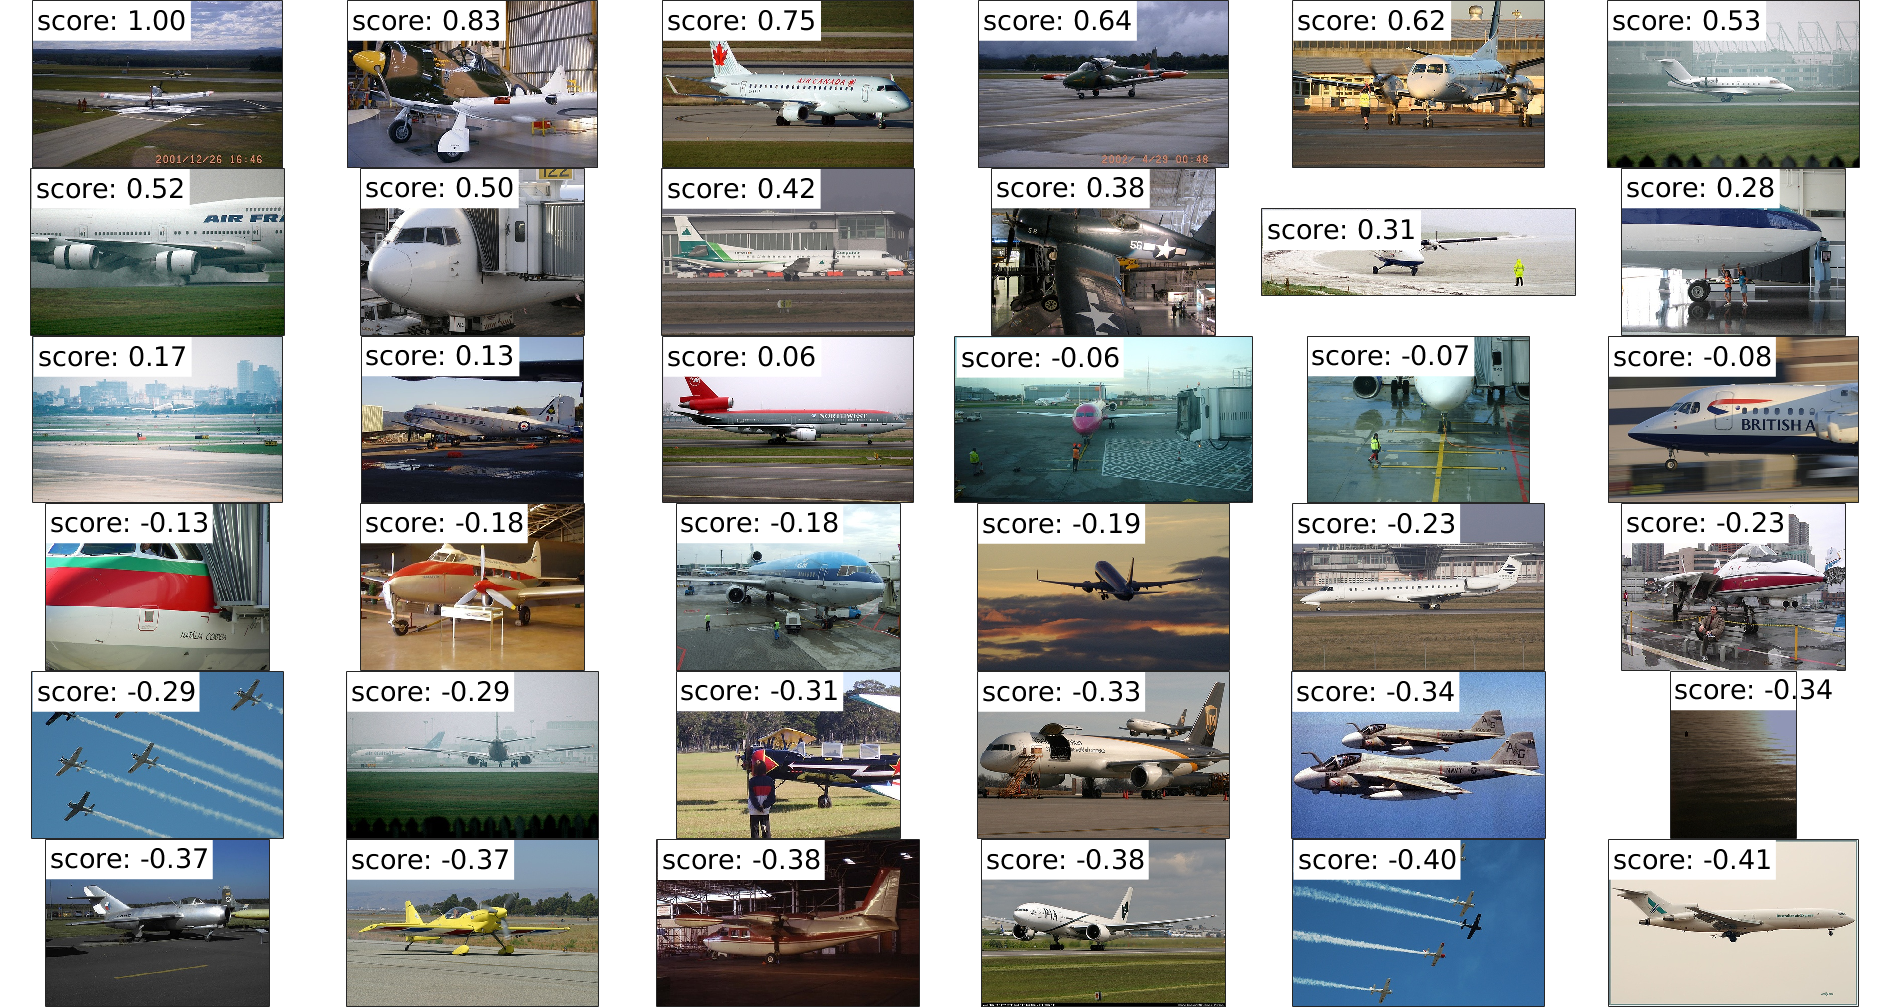
\includegraphics[width = 1.0\textwidth]{1B1_C_10}
	\caption{Ranking of a subset of 36 training images with \( C = 10\)}
	\label{fig_1B1}
\end{figure}
A subset of \(36\) training images is ranked in figure~\ref{fig_1B1}, with the score of each one, as computed by the learned SVM classifier for a value of the regularization parameter C of \(10\). It should be noticed that the indicated score is only qualitative, and has to be compared with the score of another image, \textit{i.d} images should be ranked in function of their respective score.

\clearpage
\question{QB2: In your report, show relevant patches for the three most relevant visual words (in three separate figures) for the top ranked training image. Are the most relevant visual words on the airplane or also appear on background?}

\begin{figure}[ht!]
	\centering
	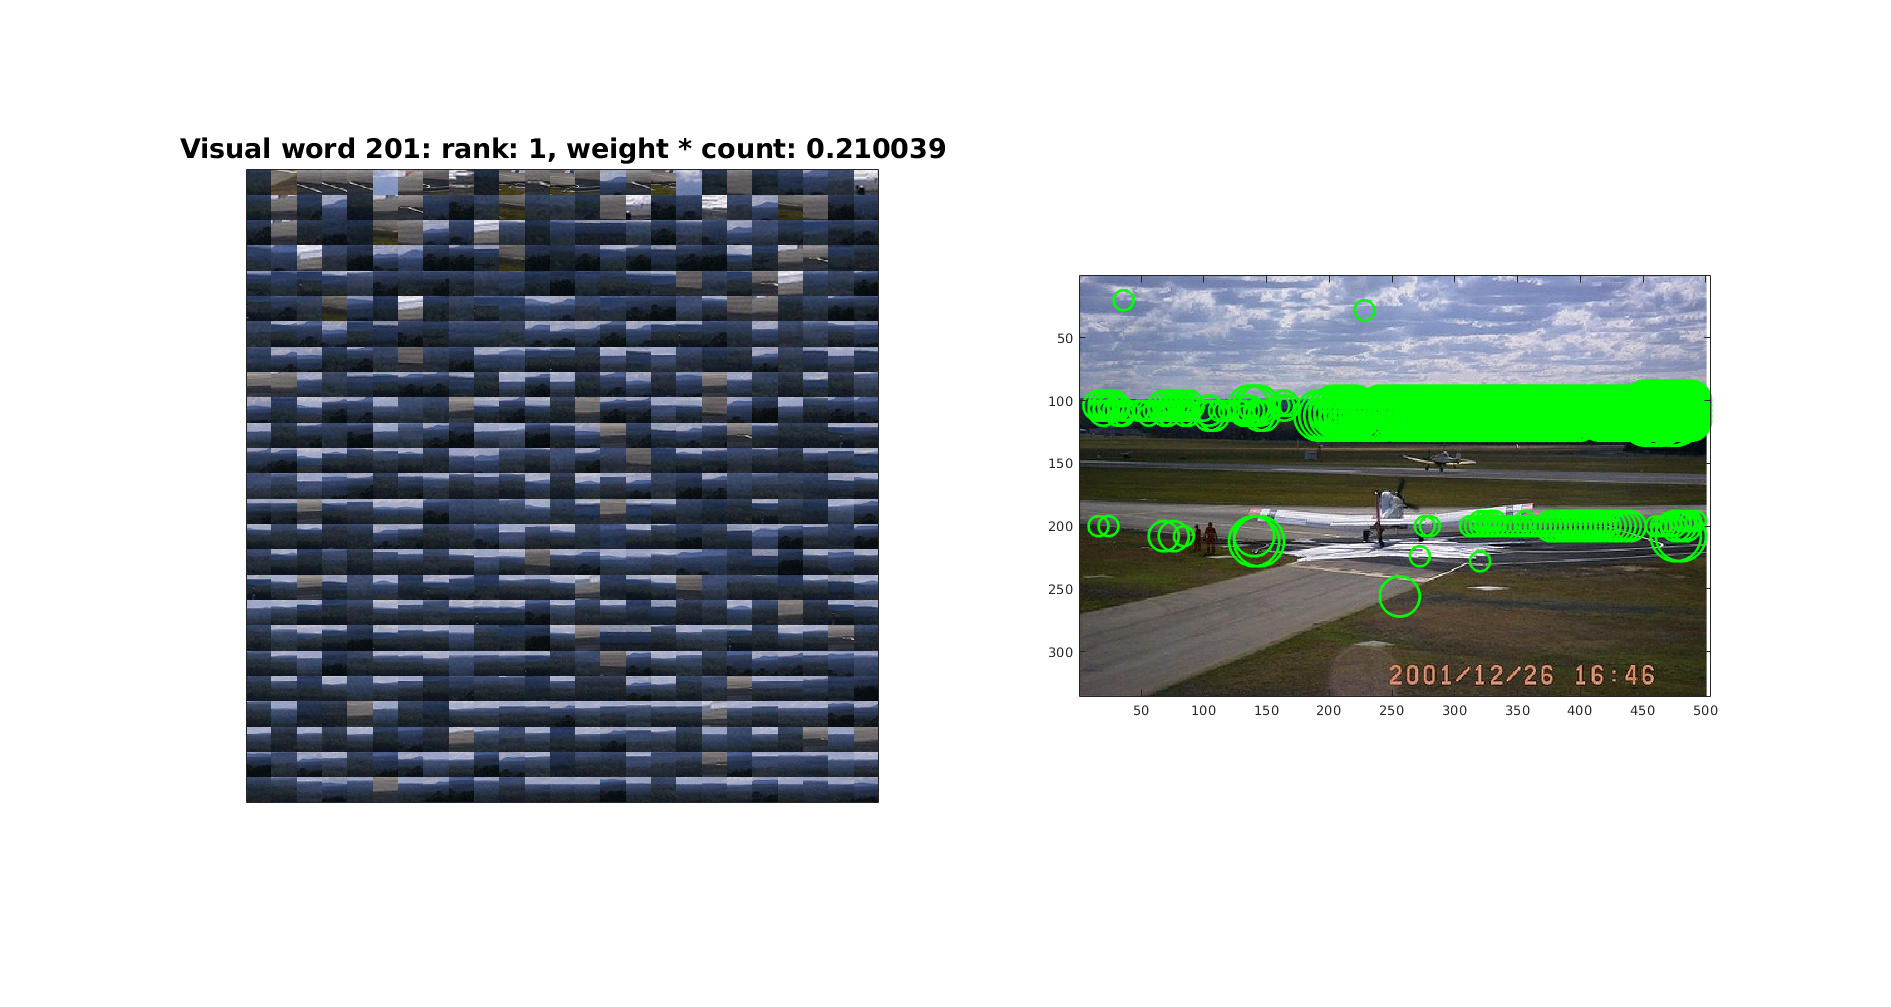
\includegraphics[width = 1.0\textwidth]{1B2_vw_1}
	\caption{Relevant patches for the first most relevant visual word and for the first ranking image of the same subset as in figure~\ref{fig_1B1}, and their positions in the image}
	\label{fig_1B2_vw_1}
\end{figure}

\begin{figure}[ht!]
	\centering
	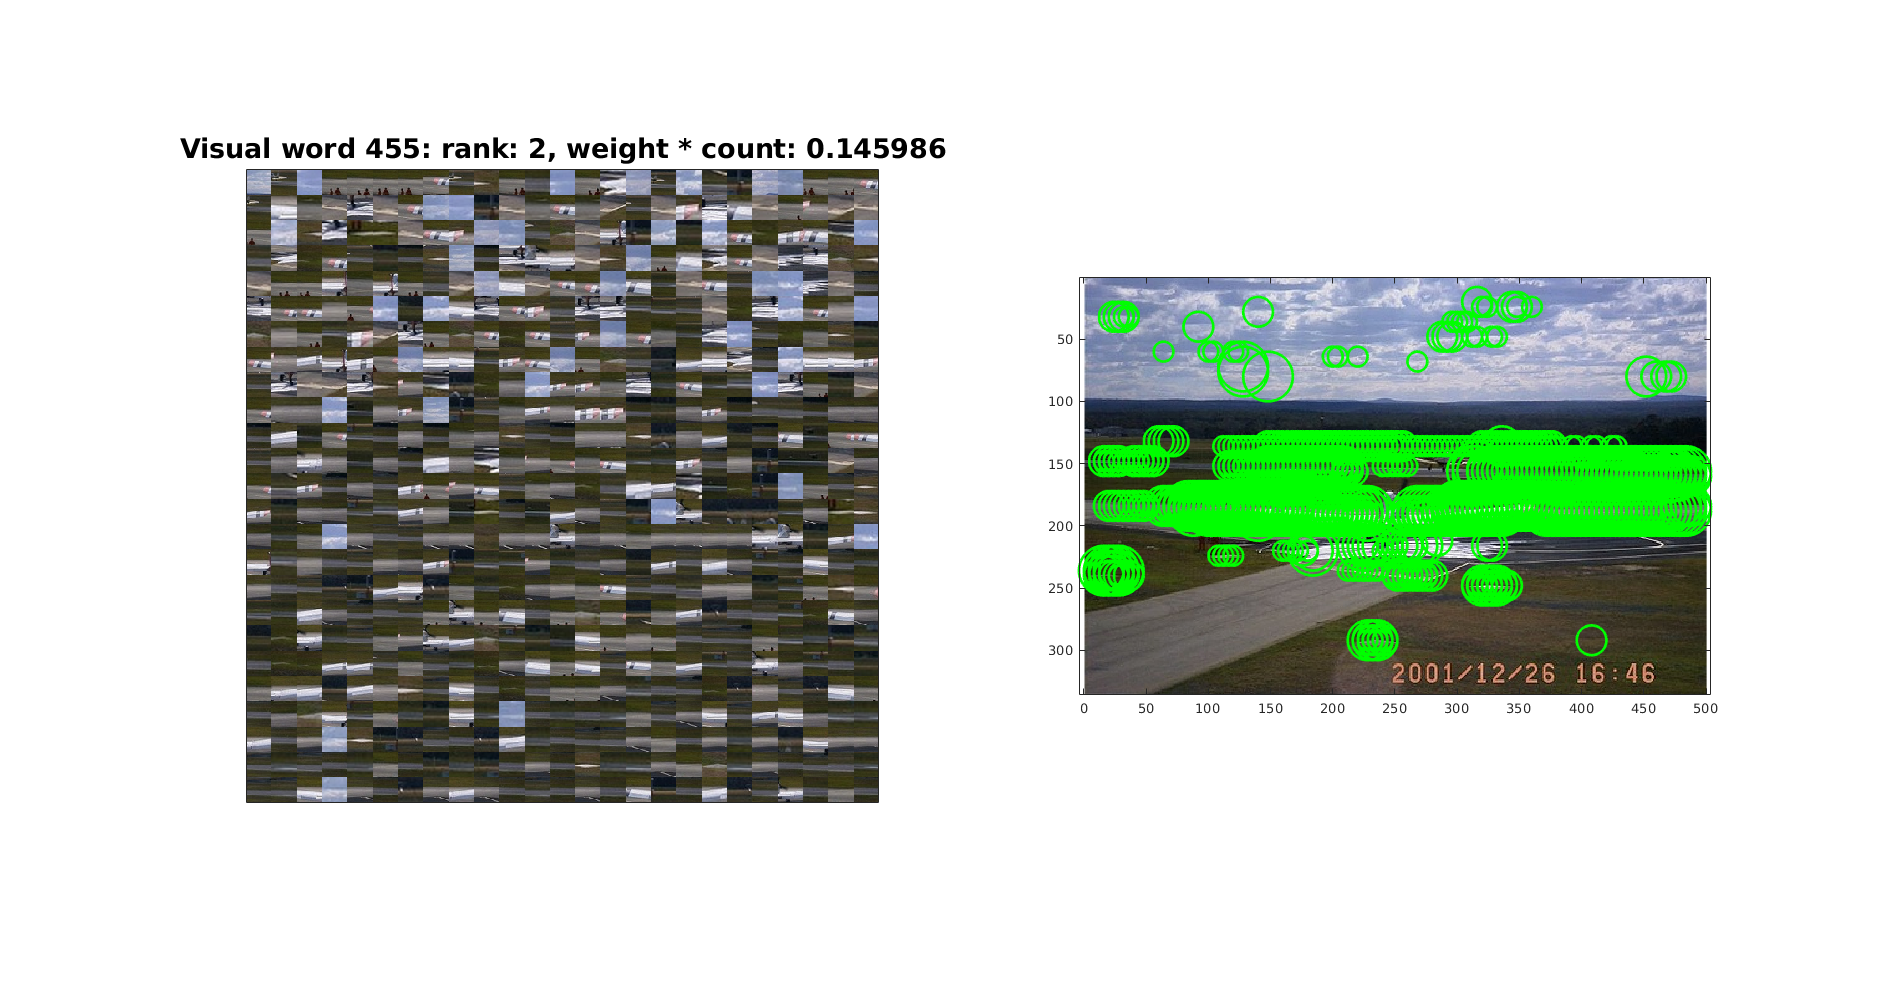
\includegraphics[width = 1.0\textwidth]{1B2_vw_2}
	\caption{Relevant patches for the second most relevant visual word and for the first ranking image of the same subset as in figure~\ref{fig_1B1}, and their positions in the image}
	\label{fig_1B2_vw_2}
\end{figure}

\begin{figure}[ht!]
	\centering
	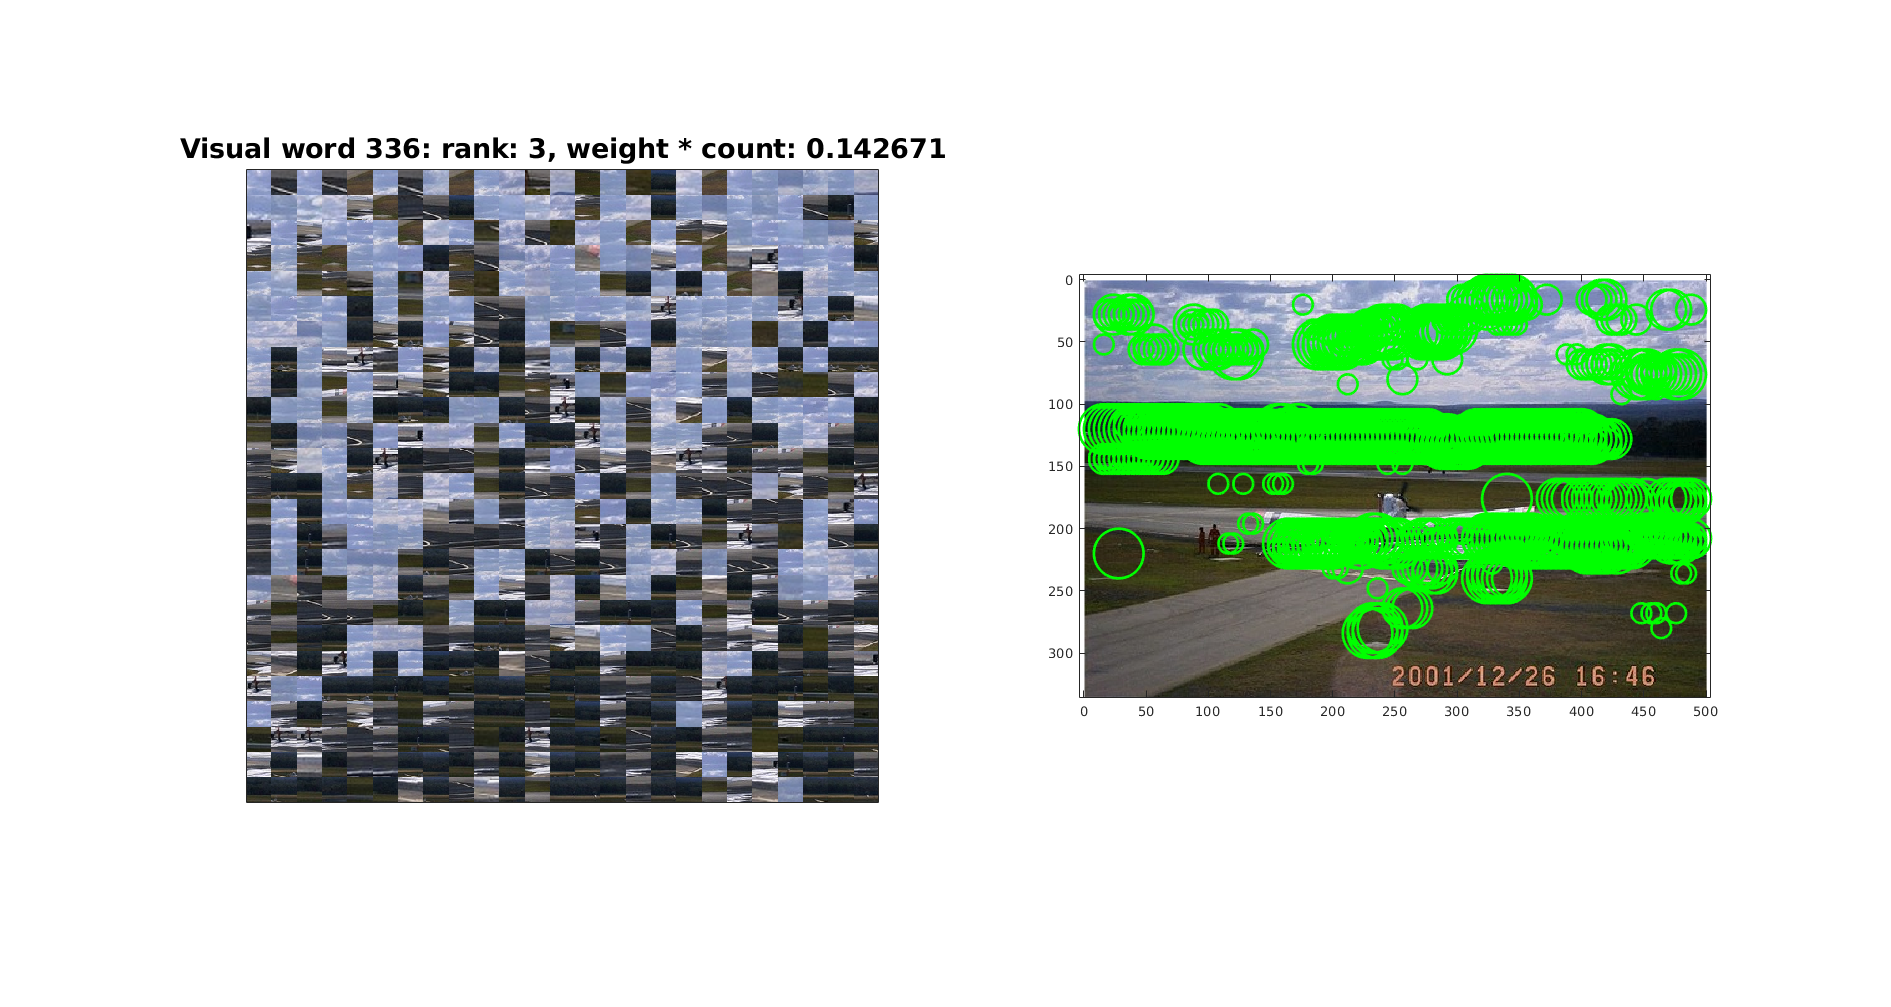
\includegraphics[width = 1.0\textwidth]{1B2_vw_3}
	\caption{Relevant patches for the third most relevant visual word and for the first ranking image of the same subset as in figure~\ref{fig_1B1}, and their positions in the image}
	\label{fig_1B2_vw_3}
\end{figure}

In figures~\ref{fig_1B2_vw_1}~\ref{fig_1B2_vw_2}~\ref{fig_1B2_vw_3}, the patches associated to the first three most relevant visual words are shown, with their positions on the first ranked image of the subset as shown in figure~\ref{fig_1B1}. It is important to notice, as shown in the three figures, in patches and in their locations, that the three most relevant visual words are essentially located in the background, in the forest in figure~\ref{fig_1B2_vw_1}, in the tarmac in figure~\ref{fig_1B2_vw_2}, in the sky in figure~\ref{fig_1B2_vw_3}, and not in the airplane.

\clearpage

\section{Classify the test images and assess the performance}

\question{QC1: Why is the bias term not needed for the image ranking?}

In the image ranking, the bias is a constant term, wich doesn't change the ranks. It's then not needed. The important part is the \( w^{\intercal} \cdot h\).

\section{Learn a classifier for the other classes and assess its performance}

\question{QD1: In your report, show the top ranked images, precision-recall curves and APs for the test data of all the three classes (aeroplanes, motorbikes, and persons). Does the AP performance for the different classes match your expectations based on the variation of the class images?}

In figures~\ref{fig_1D1_aeroplanes}~\ref{fig_1D1_motorbikes}~\ref{fig_1D1_persons} are shown the SVM classifier learnt respectively on classes aeroplanes, motorbikes and persons. It's interesting to notice that the AP value is quite similar between the aeroplanes (\(54.95~\%\)) and the motorbikes (\(48.66~\%\)) class, when the AP value for the persons class is much higher (\(70.64~\%\)). This fact can be explain by the inner-class variation, which is reasonably smaller for the persons because of their face, which is approximately constant in shape for every human. On the other hand, the aeroplanes and motorbikes can vary, for the first in term of paintings, and for the second in term of shape and paintings in between wheels. The paintings (= inner-class variations) change may be interpreted as change in gradients directions and values for SIFT descriptors, and therefore for change in visual words.

\begin{figure}[ht!]
	\centering
	\begin{subfigure}[b]{\textwidth}
		\centering
		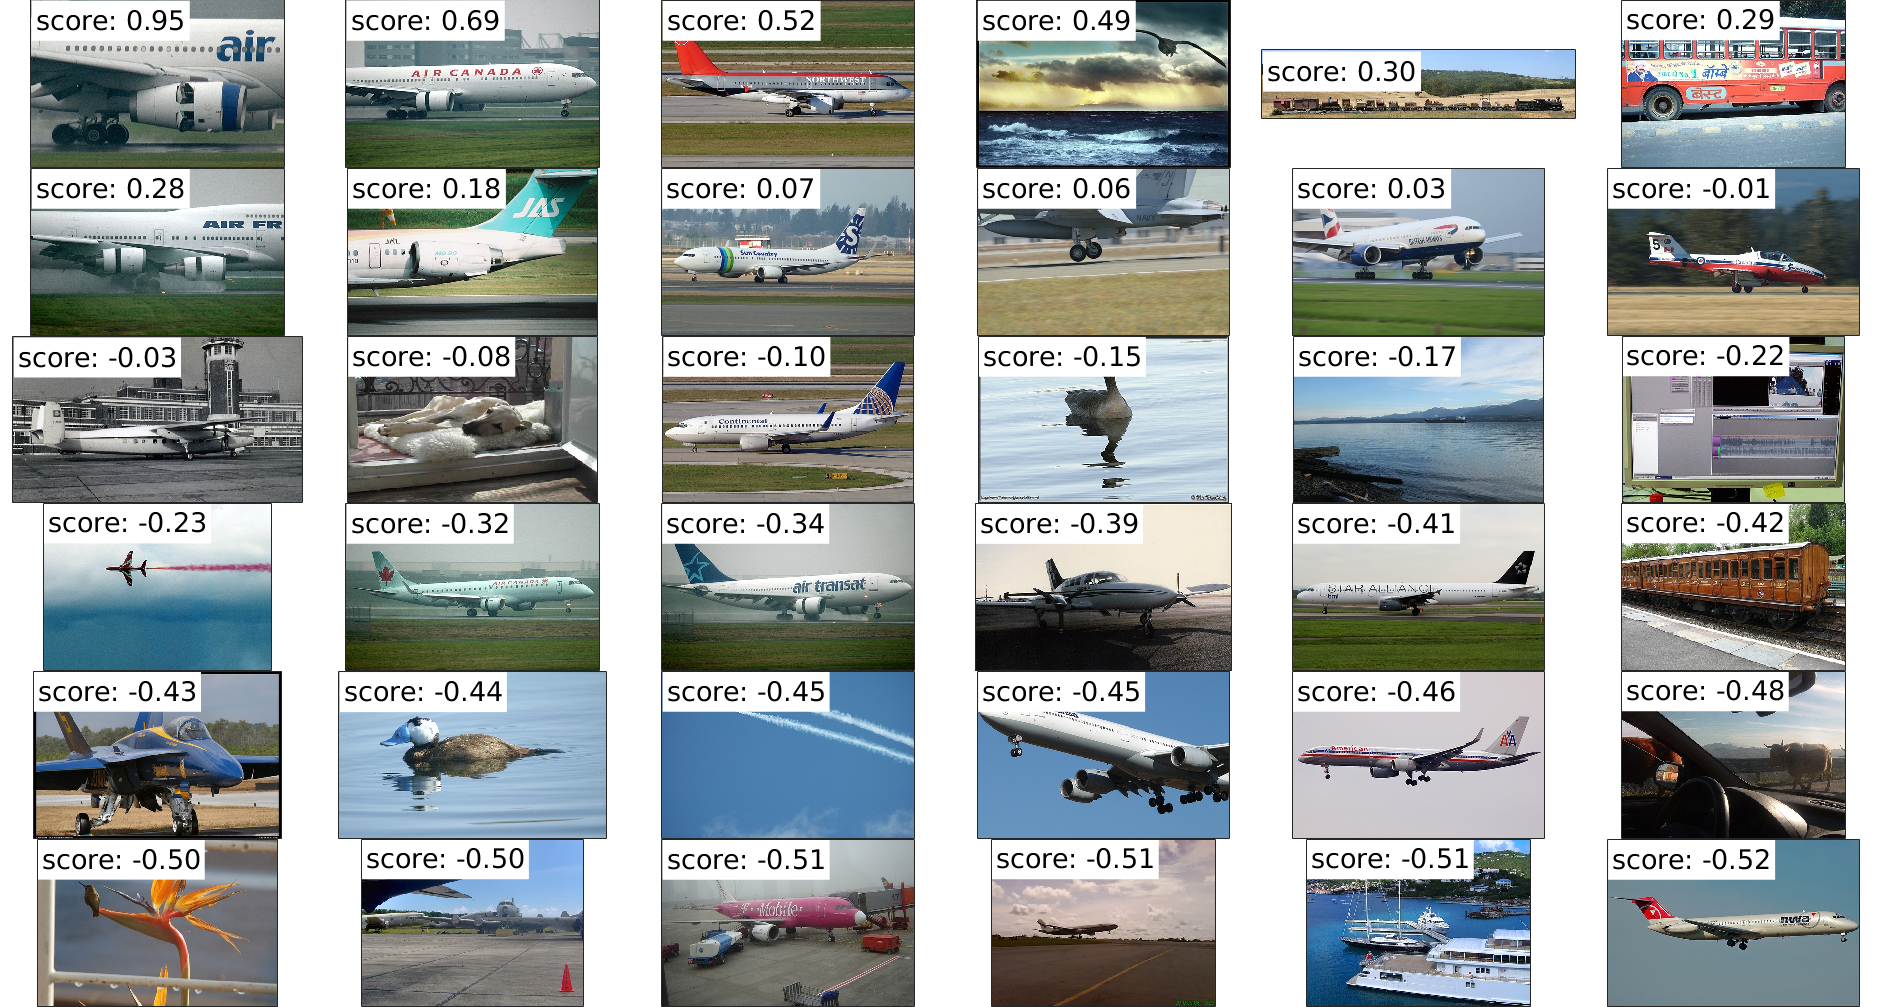
\includegraphics[width = 1.0\textwidth]{1D1_aeroplanes_C_10}
		\subcaption{Ranking of a subset of 36 testing images with \( C = 10\) : \(24\) over \(36\) images are correctly retrieved.}
		\label{fig_1D1_aeroplanes_a}
	\end{subfigure}
	\begin{subfigure}[b]{0.8\textwidth}
		\centering
		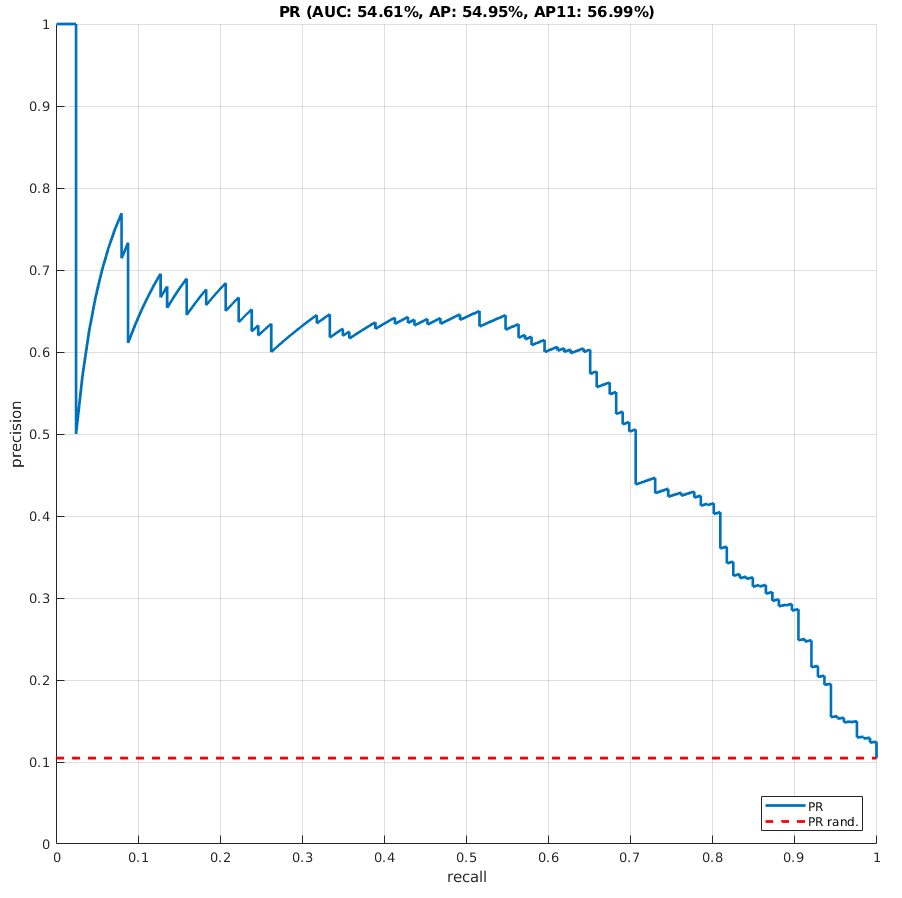
\includegraphics[width = 1.0\textwidth]{1D1_aeroplanes_AP_test_C_10}
		\subcaption{Precision-recall curve for the test data. \(AP = 54.95~\%\)}
		\label{fig_1D1_aeroplanes_b}
	\end{subfigure}
	\caption{SVM Classifier learnt for aeroplanes class}
	\label{fig_1D1_aeroplanes}
\end{figure}

\begin{figure}[ht!]
	\centering
	\begin{subfigure}[b]{\textwidth}
		\centering
		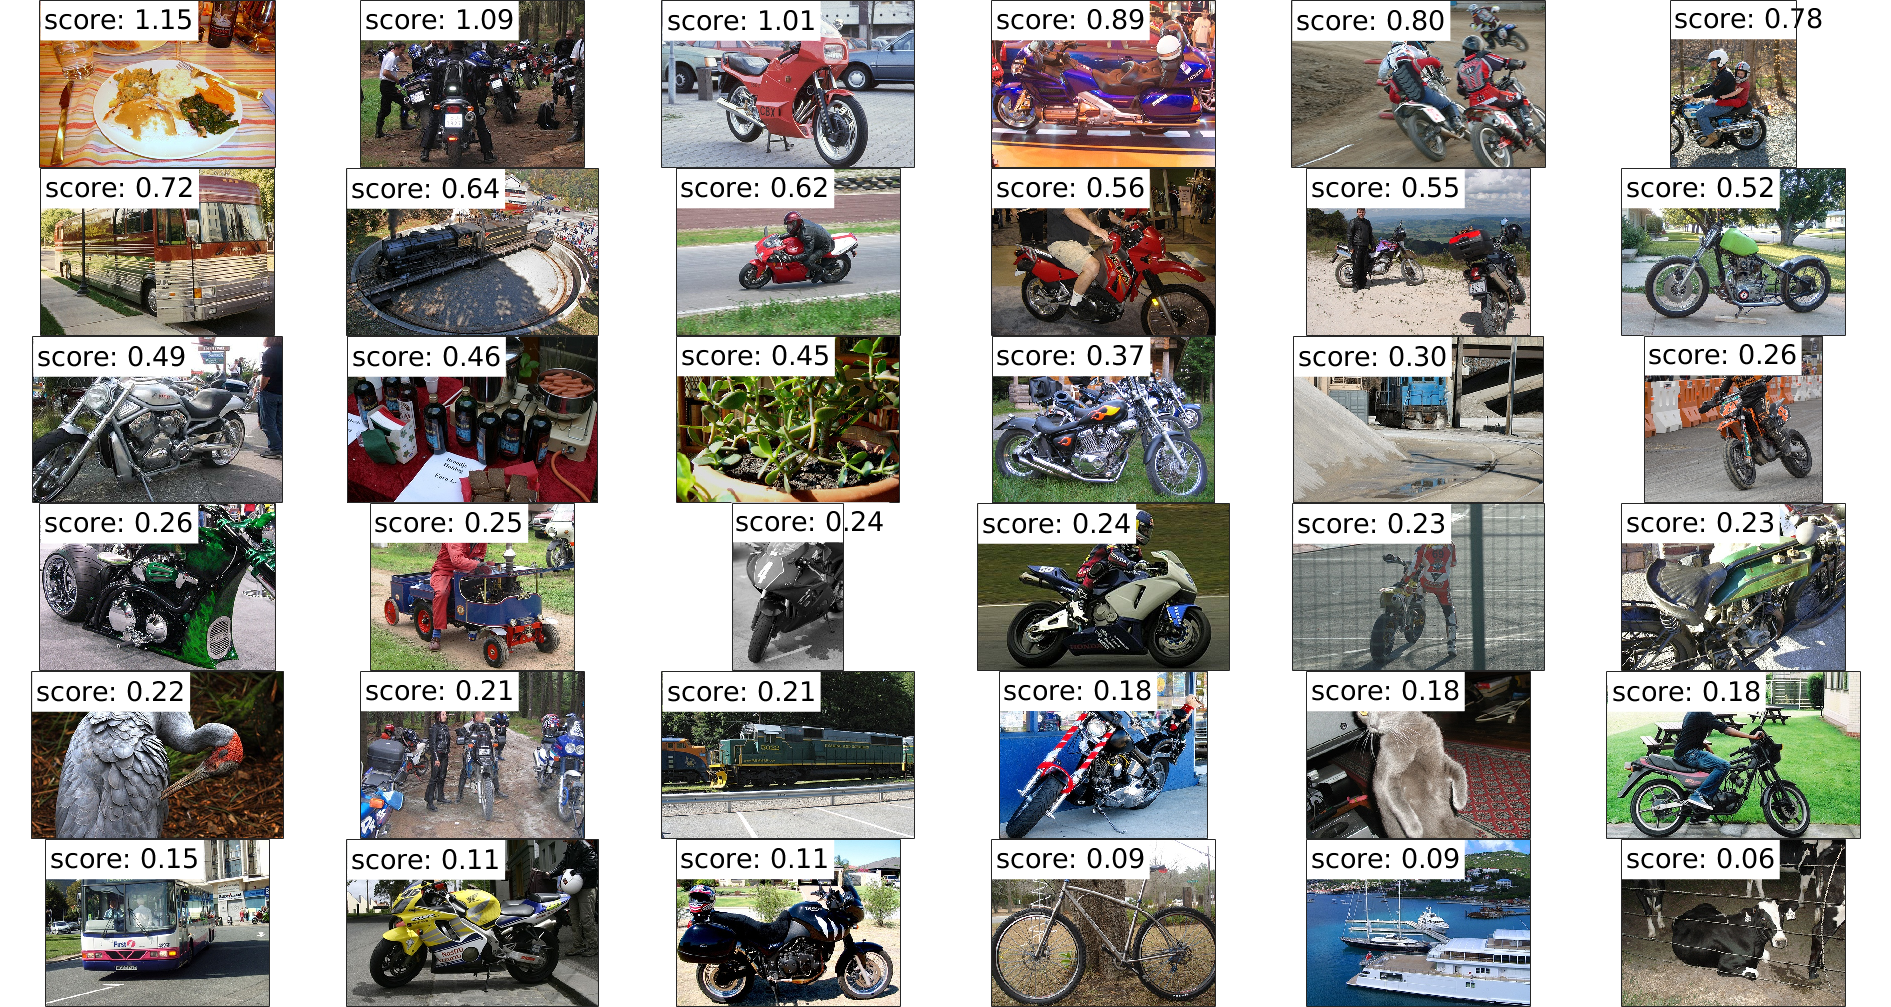
\includegraphics[width = 1.0\textwidth]{1D1_motorbikes_C_10}
		\subcaption{Ranking of a subset of 36 testing images with \( C = 10\) : \(24\) over \(36\) images are correctly retrieved.}
		\label{fig_1D1_motorbikes_a}
	\end{subfigure}
	\begin{subfigure}[b]{0.8\textwidth}
		\centering
		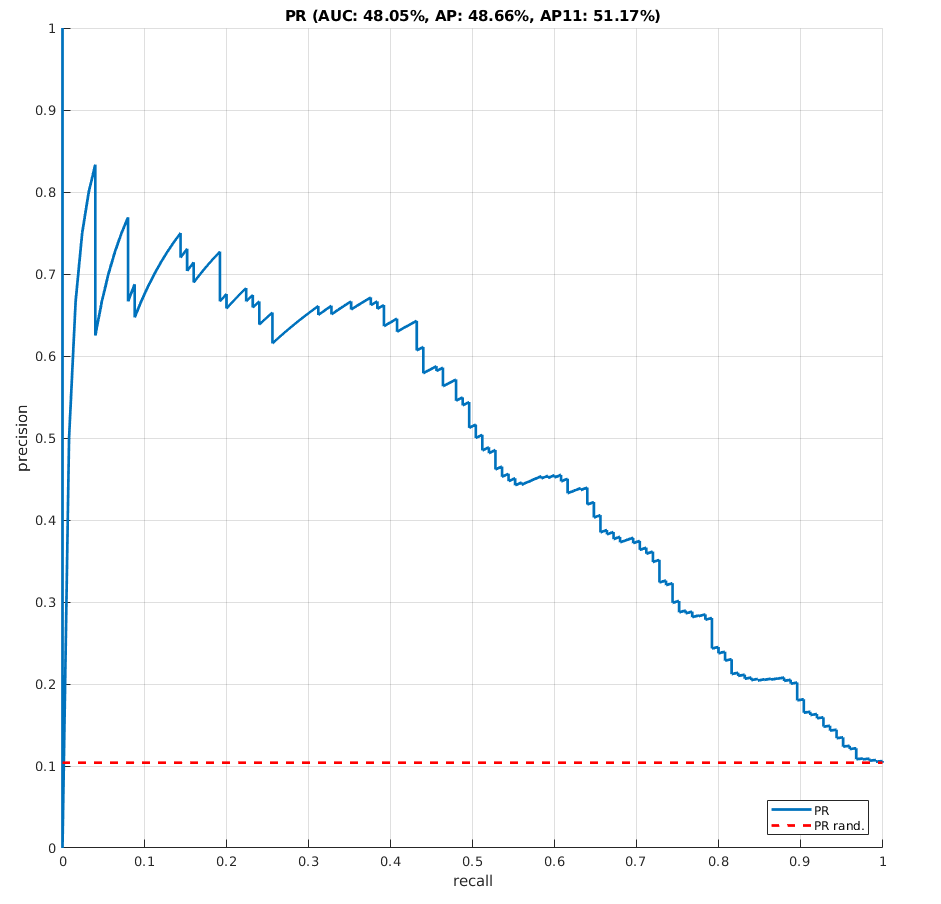
\includegraphics[width = 1.0\textwidth]{1D1_motorbikes_AP_test_C_10}
		\subcaption{Precision-recall curve for the test data. \(AP = 48.66~\%\)}
		\label{fig_1D1_motorbikes_b}
	\end{subfigure}
	\caption{SVM Classifier learnt for motorbikes class}
	\label{fig_1D1_motorbikes}
\end{figure}

\begin{figure}[ht!]
	\centering
	\begin{subfigure}[b]{\textwidth}
		\centering
		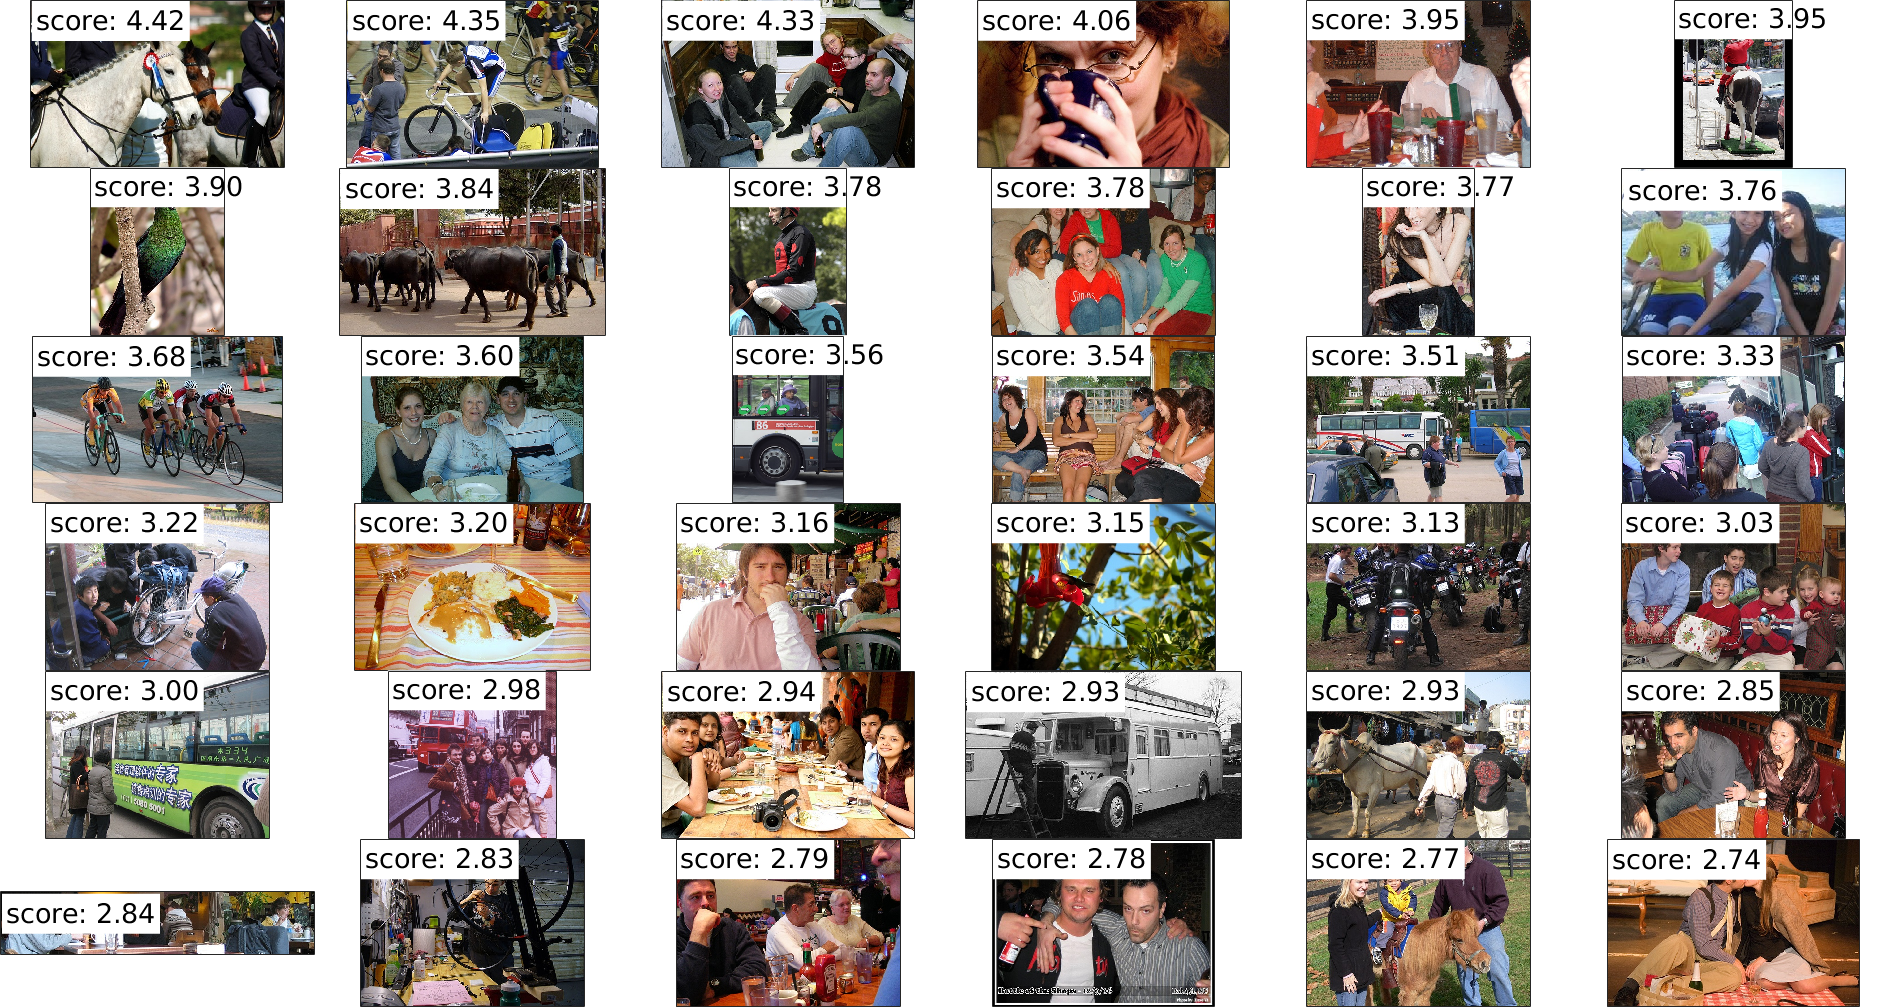
\includegraphics[width = 1.0\textwidth]{1D1_persons_C_10}
		\subcaption{Ranking of a subset of 36 testing images with \( C = 10\) : \(33\) over \(36\) images are correctly retrieved.}
		\label{fig_1D1_persons_a}
	\end{subfigure}
	\begin{subfigure}[b]{0.8\textwidth}
		\centering
		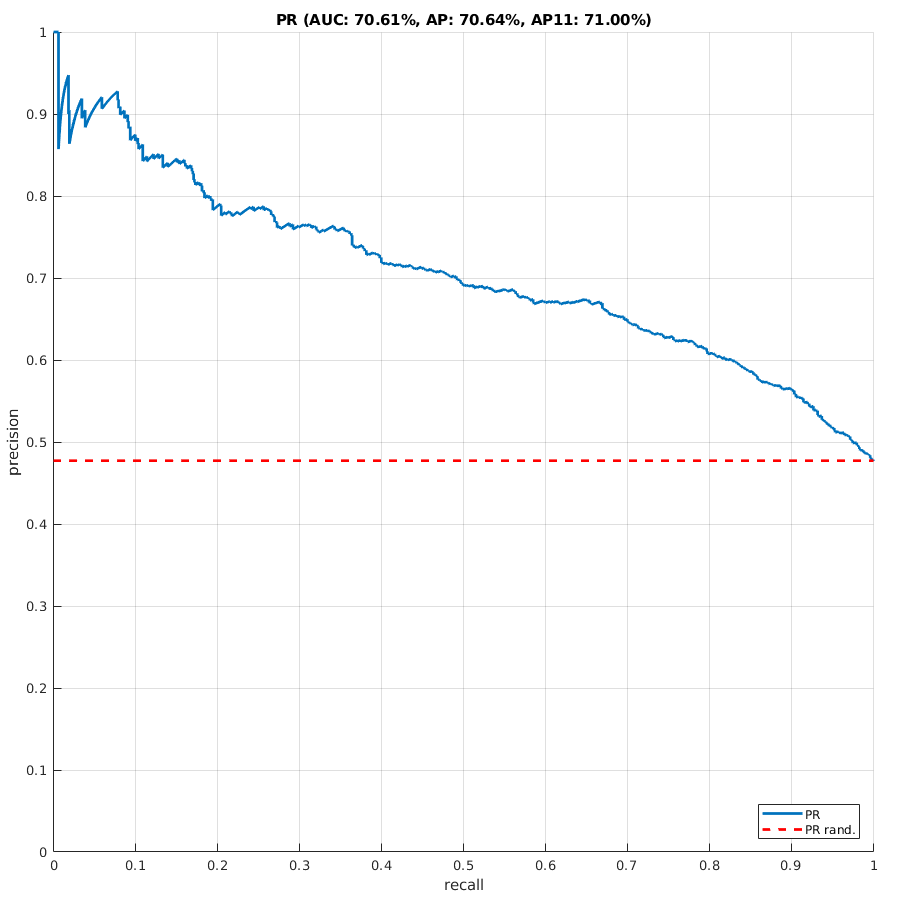
\includegraphics[width = 1.0\textwidth]{1D1_persons_AP_test_C_10}
		\subcaption{Precision-recall curve for the test data. \(AP = 70.64~\%\)}
		\label{fig_1D1_persons_b}
	\end{subfigure}
	\caption{SVM Classifier learnt for persons class}
	\label{fig_1D1_persons}
\end{figure}

\clearpage
\question{QD2: For the motorbike class, give the rank of the first false positive image. What point on the precision-recall curve corresponds to this first false positive image? Give in your report the value of precision and recall for that point on the precision-recall curve.}

For the motorbike class, the first false positive image, visible in figure~\ref{fig_1D1_motorbikes_a}, is the top scoring one (\textit{006687.jpg}), which corresponds to the point \( (Recall(2), Precision(2)) = (0,0)\) on the precision-recall curve, \textit{i.e.} the first point of the precision-recall curve, after the conventional  \( (Recall(1), Precision(1)) = (0,1)\).

\section{Vary the image representation}

\question{QE1: Include in your report precision recall-curves and APs, and compare the test performance to the spatially tiled representation in stage D. How is the performance changing? Why?}

\begin{figure}[ht!]
	\centering
	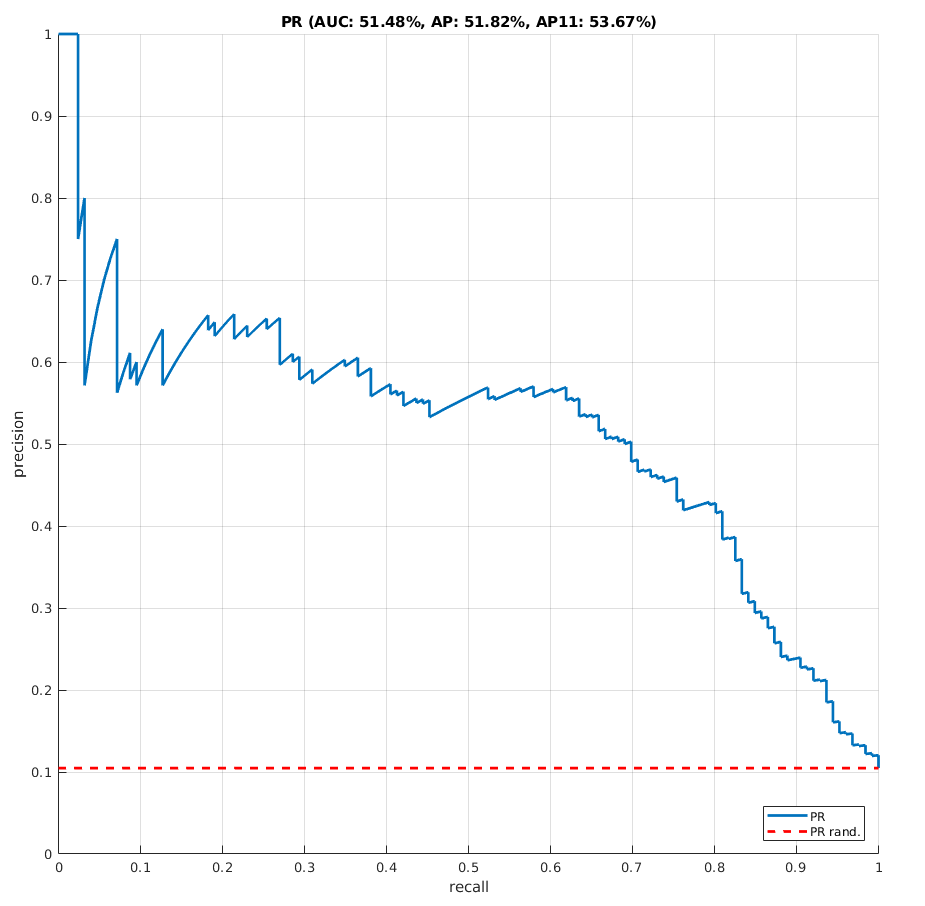
\includegraphics[width = 1.0\textwidth]{1E1_aeroplanes_AP_test_C_10}
	\caption{SVM Classifier learnt for aeroplanes class : Precision-recall curve for the test data. \(AP = 51.82~\%\)}
	\label{fig_1E1_aeroplanes}
\end{figure}

\begin{figure}[ht!]
	\centering
	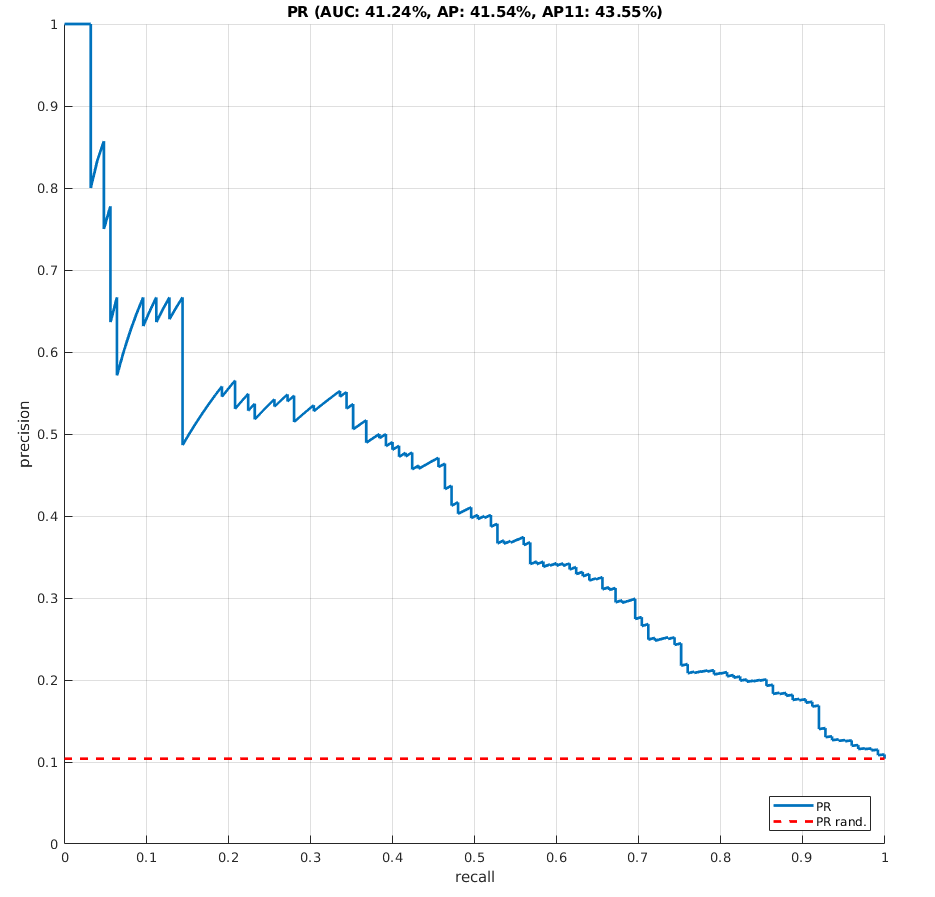
\includegraphics[width = 1.0\textwidth]{1E1_motorbikes_AP_test_C_10}
	\caption{SVM Classifier learnt for motorbikes class : Precision-recall curve for the test data. \(AP = 41.54~\%\)}
	\label{fig_1E1_motorbikes}
\end{figure}

\begin{figure}[ht!]
	\centering
	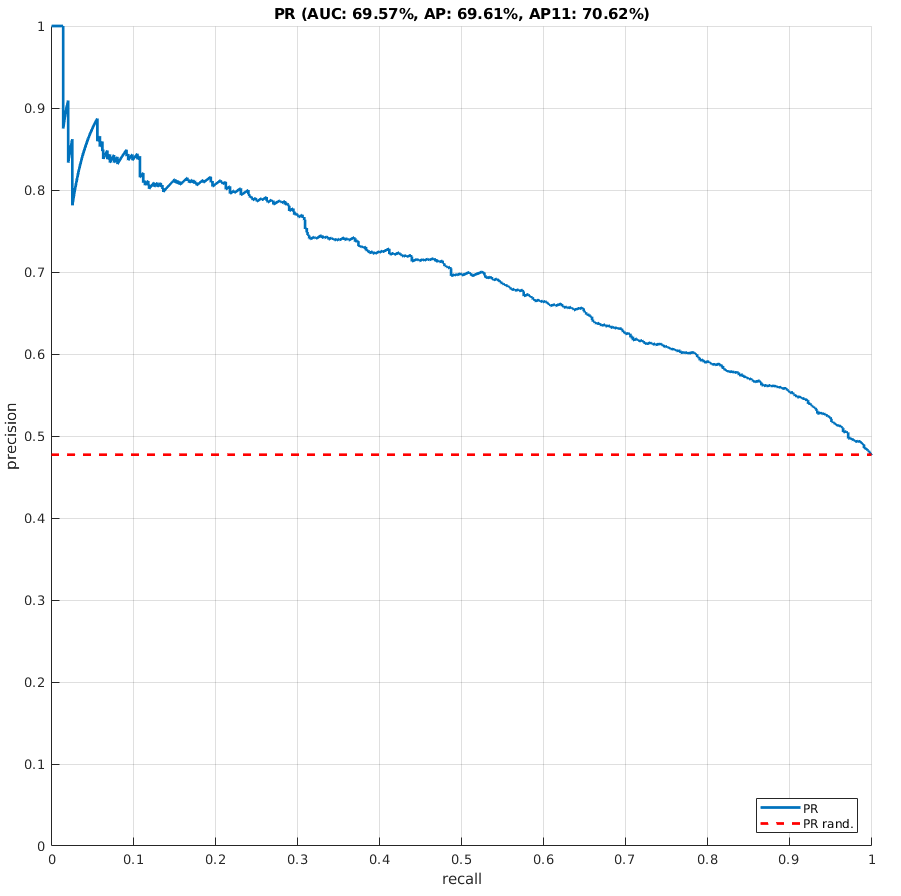
\includegraphics[width = 1.0\textwidth]{1E1_persons_AP_test_C_10}
	\caption{SVM Classifier learnt for persons class : Precision-recall curve for the test data. \(AP = 69.61~\%\)}
	\label{fig_1E1_persons}
\end{figure}

For the three classes, the AP value decreases respectively by \(3~\%\),  \(7~\%\) and \(1~\%\) for aeroplanes, motorbikes and persons. These variations are class dependants, meaning that the spatial information brought by the spatial tiling is more relevant for the motorbikes, then for aeroplanes and finaly for persons. This might be correlated with the inner-class variation, as the decrease is inverse-proportional to the initial AP-value.

\clearpage

\question{QE2: Modify exercise1.m to use L1 normalization and no normalization and measure the performance change.}

In table~\ref{tab_normalization} is shown the effect of different normalizations over the AP value of the classifier. We can notice that the effect of the normalization differs for the 3 classes. For aeroplanes, the \(L_1\) norm produces better AP value than without normalization. But the \(L_2\) norm produces even worst AP value. For motorbikes, the effect of normalization is quite null whereas for the persons class, the \(L_2\) norm produces better AP value than the others. To conclude, it seems that the performance may be affected by the normalization process, but not in a uniform way.

\begin{table}[ht!]
	\centering
	\begin{tabular}{|l | p{3.5cm} | p{3.5cm}| p{3.5cm}|}
		\hline
		Class      & AP in test tiling with \(L_2\) norm & AP in test tiling with \(L_1\) norm & AP in test tiling without normalization \\\hline\hline
		Aeroplanes & \(54.95~\%\)                        & \(64.60~\%\)                        & \(62.45~\%\)                            \\\hline
		Motorbikes & \(48.66~\%\)                        & \(48.70~\%\)                        & \(48.73~\%\)                            \\\hline
		Persons    & \(70.64~\%\)                        & \(67.37~\%\)                        & \(67.20~\%\)                            \\\hline
	\end{tabular}
	\caption{Effect of histogram normalization over classifier performance}
	\label{tab_normalization}
\end{table}


\question{QE3: What can you say about the self-similarity, \(K(h,h)\), of a BoVW histogram h that is L2 normalized? Hint: Compare \(K(h,h)\) to the similarity, \(K(h,h'\)), of two different L2 normalized BoVW histograms \(h\) and \(h'\).
	Can you say the same for unnormalized or L1 normalized histograms?}

For \(L_2\) normalized BoVW, the following inequality holds :
\[
	K(h,h') \leq K(h,h)
\]
This one doesn't hold for \(L_1\) normalized or unnormalized histograms.

\question{QE4: Do you see a relation between the classification performance and L2 normalization?}



\section{Vary the classifier}

\question{QF1: Based on the rule of thumb introduced above, how should the BoVW histograms \(h\) and \(h'\) be normalized? Should you apply this normalization before or after taking the square root?}

Based on the previous rule of thumb, the histograms should be normalized before fedding the SVM, that means, after the square root of histogram has to be normalized.

\question{QF2: Why is this procedure equivalent to using the Hellinger kernel in the SVM classifier?}

Because the SVM only depends on the dot product between the 2 histograms, which can be square rooted before the product (our procedure), or after the product in the Hellinger Kernel. In both case, the \(K(k, h')\) would be the same.

\question{QF3: Why is it an advantage to keep the classifier linear, rather than using a non-linear kernel?}

The optimization of a linear problem is faster than a non-linear one.

\question{QF4: Try the other histogram normalization options and check that your choice yields optimal performance. Summarize your finding in the report (include only mAP results, no need to include the full precision-recall curves).}

\begin{table}[ht!]
	\centering
	\begin{tabular}{|l | p{5cm} | p{5cm}|}
		\hline
		Class      & AP in test tiling with \(L_2\) norm with linear SVM & AP in test tiling with Hellinger Kernel SVM \\\hline\hline
		Aeroplanes & \(54.95~\%\)                                        & \(70.72~\%\)                                \\\hline
		Motorbikes & \(48.66~\%\)                                        & \(63.25~\%\)                                \\\hline
		Persons    & \(70.64~\%\)                                        & \(77.39~\%\)                                \\\hline
	\end{tabular}
	\caption{Effect of using an Hellinger Kernel SVM over the performance of the classifier}
	\label{tab_hellinger}
\end{table}

In table~\ref{tab_hellinger} the AP-value of the classifier learnt with the Hellinger kernel is shown. A notable increase is performed in the three classes, with \(10~\%\) to \(30~\%\) of increase in comparaison with initial results.

\section{Vary the number of training images}


\question{QG1: Report and compare performance you get with the linear kernel  and with the Hellinger kernel for the different classes and proportions of training images (10\%, 50\% and 100\%). You don’t have to report the precision-recall curves, just APs are sufficient. Plot the APs for one class into a graph, with AP on the y-axis and the proportion of training images on the x-axis. You can use the matlab function plot Plot three curves (one curve for each class) into one figure. Produce two figures, one for the linear kernel and one for the Hellinger kernel. Make sure to properly label axis (use functions xlabel and ylabel), show each curve in a different color, and have a legend (function legend) in each figure. Show the two figures in your report.}

\begin{figure}[ht!]
	\centering
	\begin{subfigure}[b]{0.60\textwidth}
		\centering
		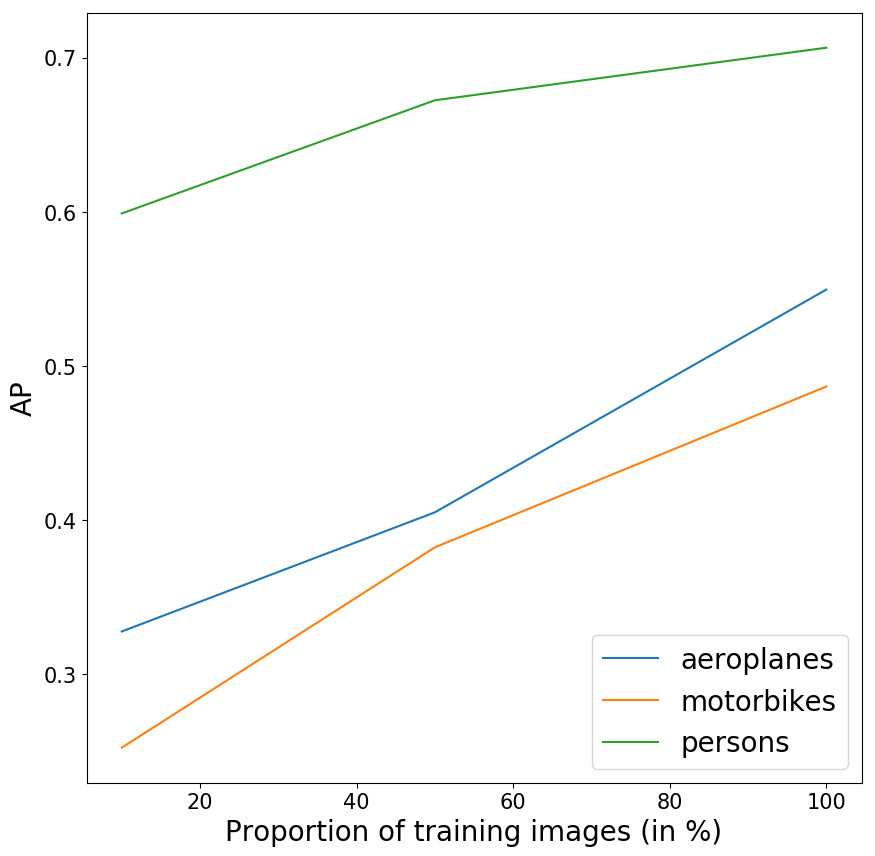
\includegraphics[width = 1.0\textwidth]{1G1_linear}
		\subcaption{With the linear kernel}
		\label{fig_1G1_a}
	\end{subfigure}
	\begin{subfigure}[b]{0.60\textwidth}
		\centering
		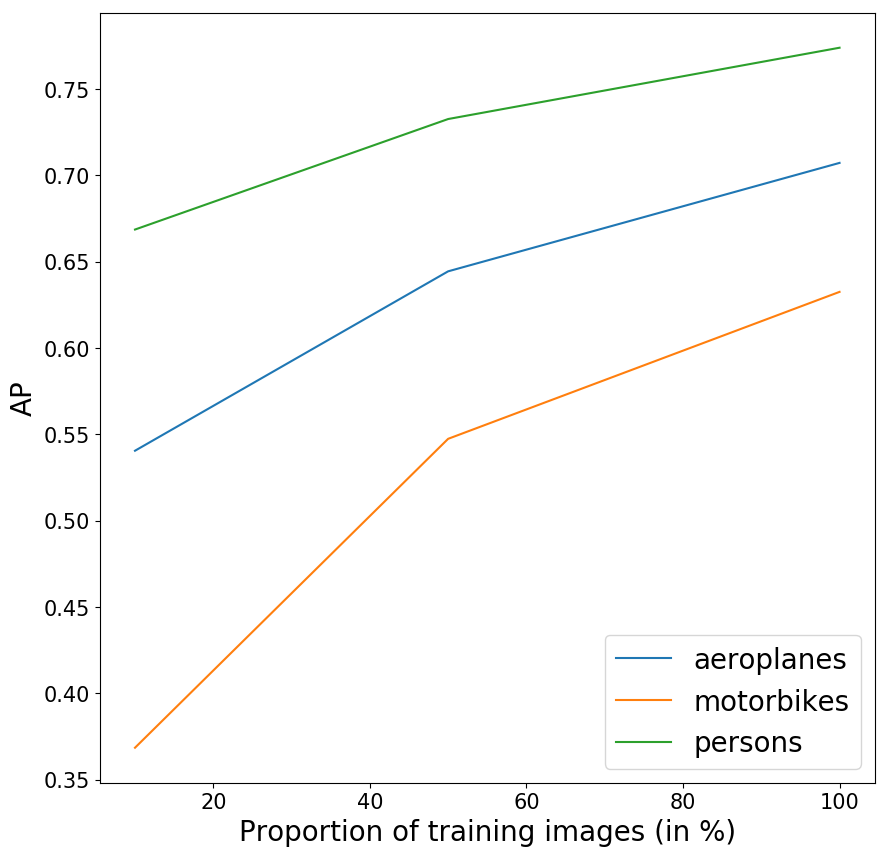
\includegraphics[width = 1.0\textwidth]{1G1_hellinger}
		\subcaption{With the Hellinger kernel}
		\label{fig_1G1_b}
	\end{subfigure}
	\caption{Effect of variations in number of training images for two different kernels in SVM classifier}
	\label{fig_1G1}
\end{figure}

In figure~\ref{fig_1G1} is presented the AP value in fuction of the kernel used and the proportion of training images used. For every proportion and every class, the AP value is higher using the Hellinger kernel.

\question{QG2: By analyzing the two figures, do you think the performance has `saturated' if all the training images are used, or would adding more training images give an improvement?}

Except for the aeroplanes in the hellinger kernel case, the increase of performance looks to decrease when close to using the totality of the training images available. But it doesn't necessary mean the saturation state is reached. Indeed, in comparison with the persons class, using 10 times more training images than the other ones, the performance is still increasing in both kernel between using 10\% of training images (equivalent in number of the 100\% in aeroplanes and motorbikes classes), and using 100\% (arround 1000 images).

\clearpage

\part{Training an Image Classifier for Retrieval using Internet image search.}

\question{QP2.1: For the horse class, report the precision at rank-36 for 5 and 10 training images. Show the training images you used. Did the performance of the classifier improve when 10 images were used?}

In figure~\ref{fig_2P2_1} are presented the training imges used.
The precision at rank-36 is :
\begin{itemize}
	\item \(3 / 36\) for 5 training images
	\item \(14 / 36\) for 10 training images
\end{itemize}
And the AP-value increases from 0.12 to 0.26. The performance of the classifier improved a lot using 5 more training images.

\begin{figure}[ht!]
	\centering
	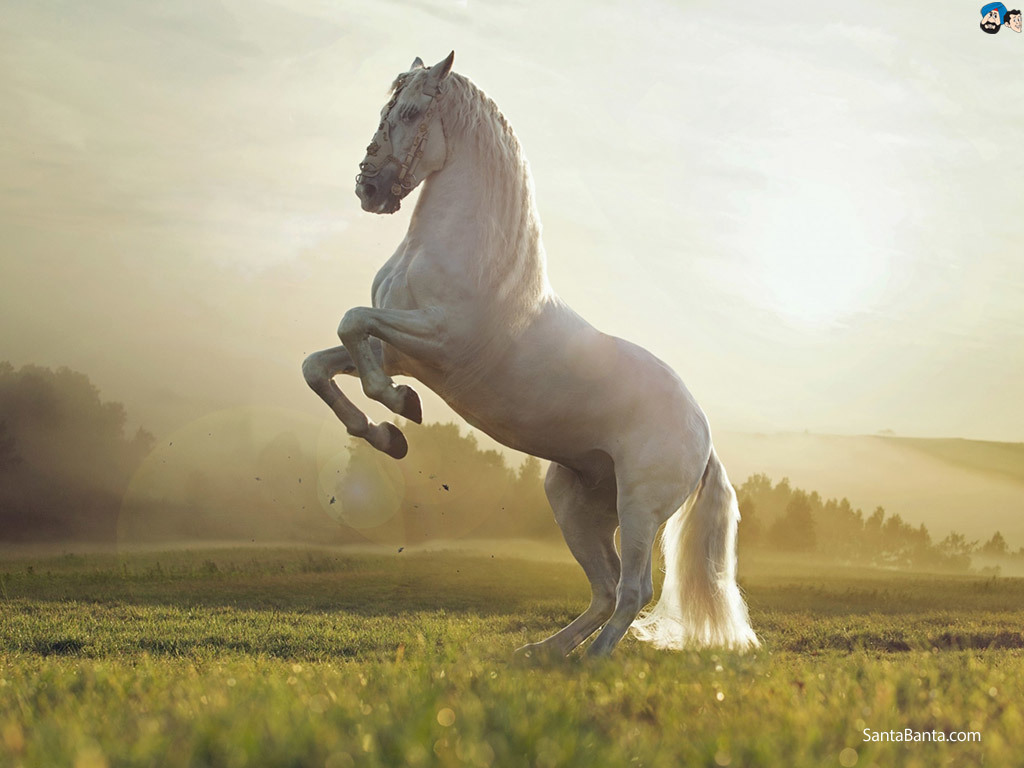
\includegraphics[height = 0.15\textheight, width = 0.4\textwidth]{horse_000001}
	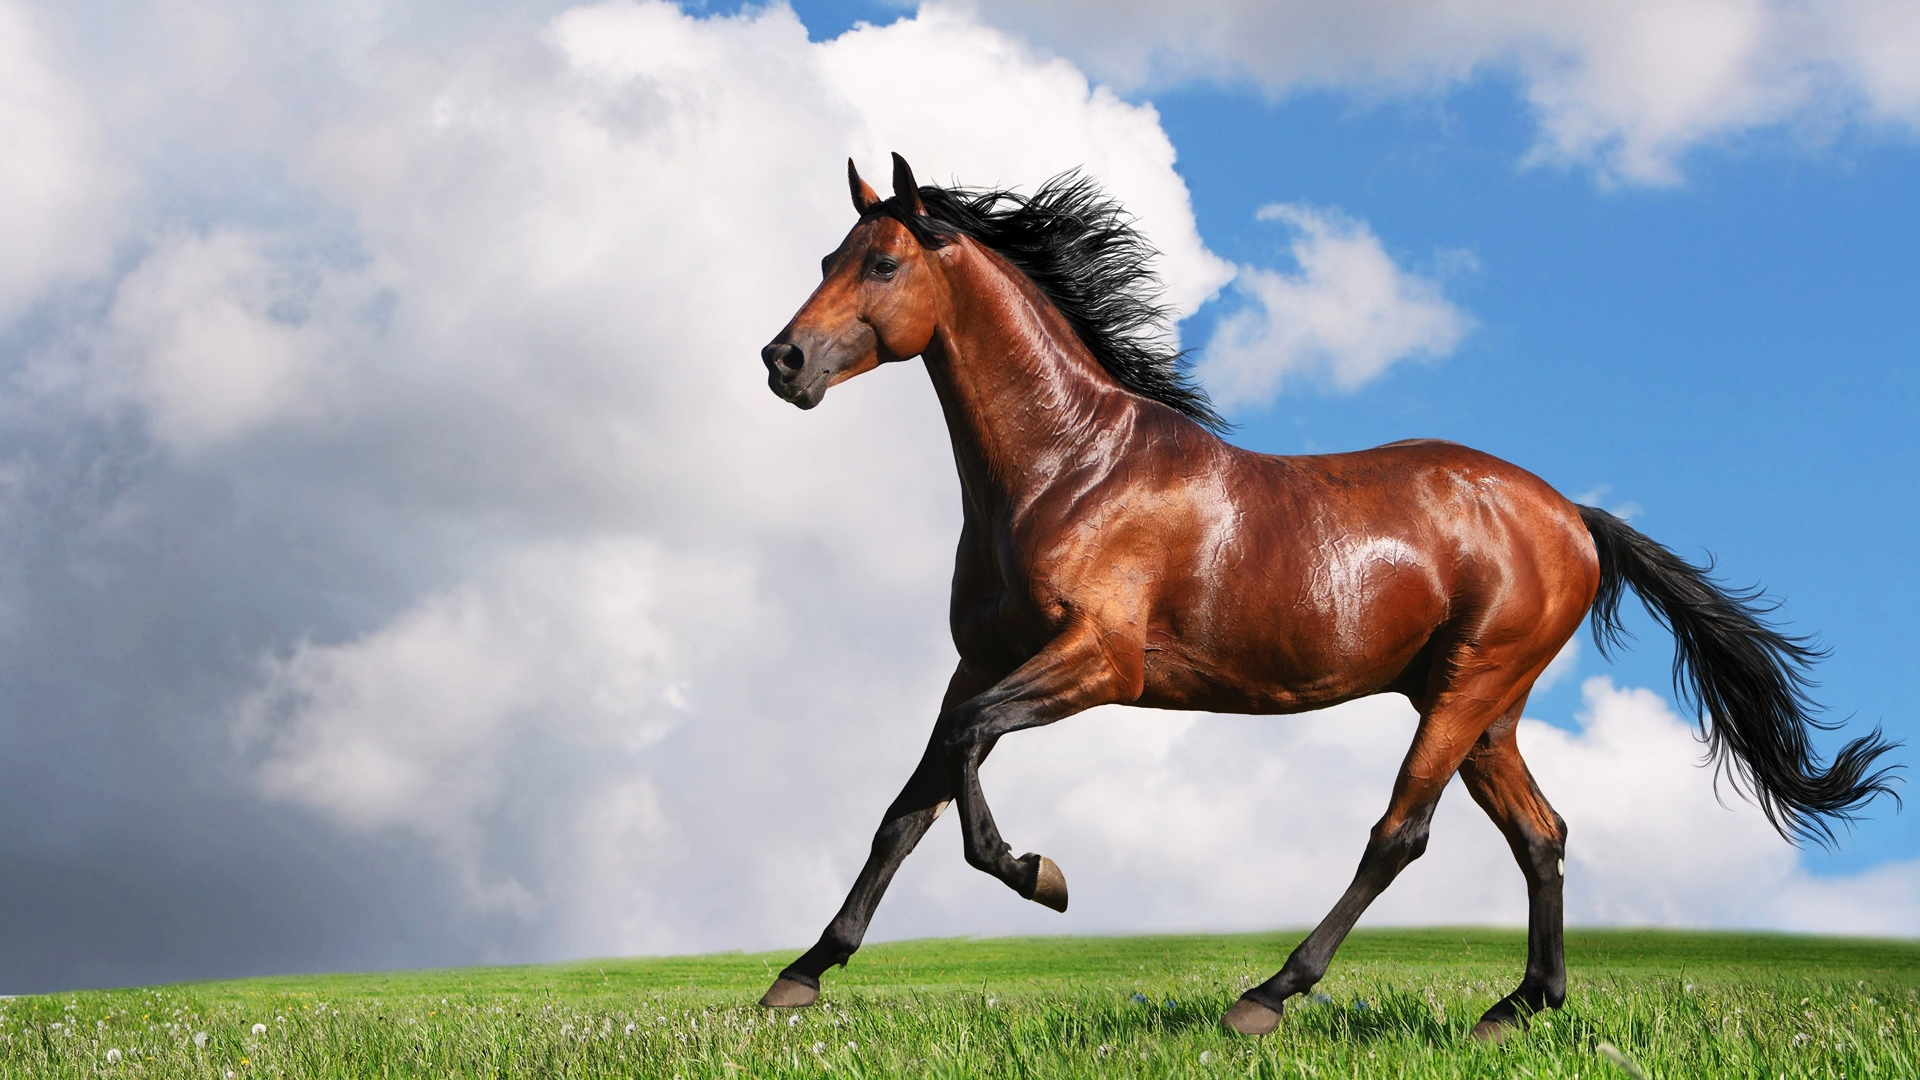
\includegraphics[height = 0.15\textheight, width = 0.4\textwidth]{horse_000002}
	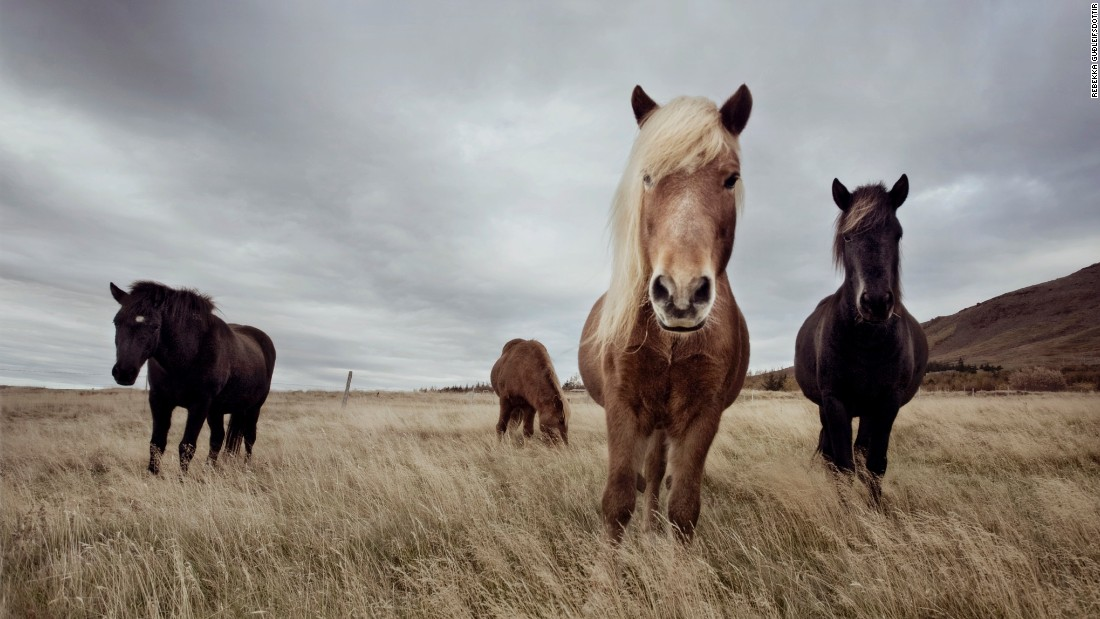
\includegraphics[height = 0.15\textheight, width = 0.4\textwidth]{horse_000003}
	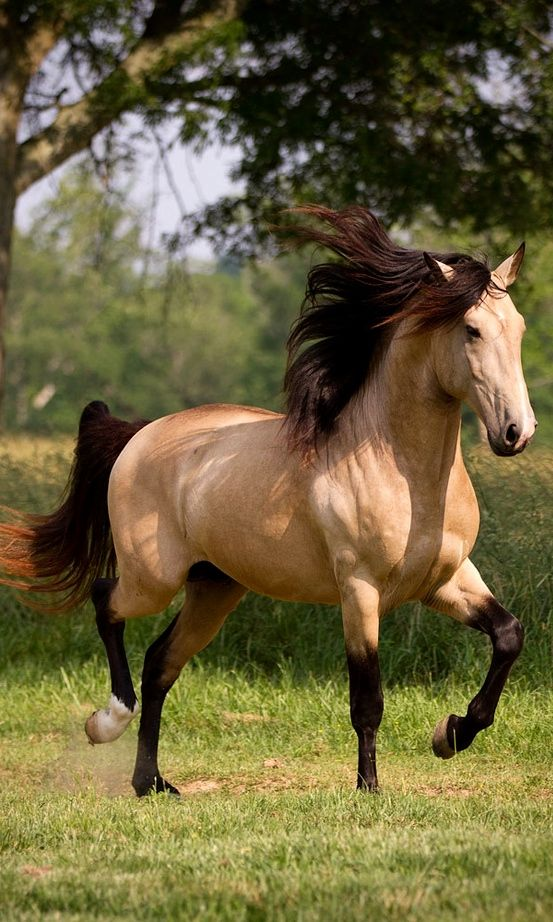
\includegraphics[height = 0.15\textheight, width = 0.4\textwidth]{horse_000004}
	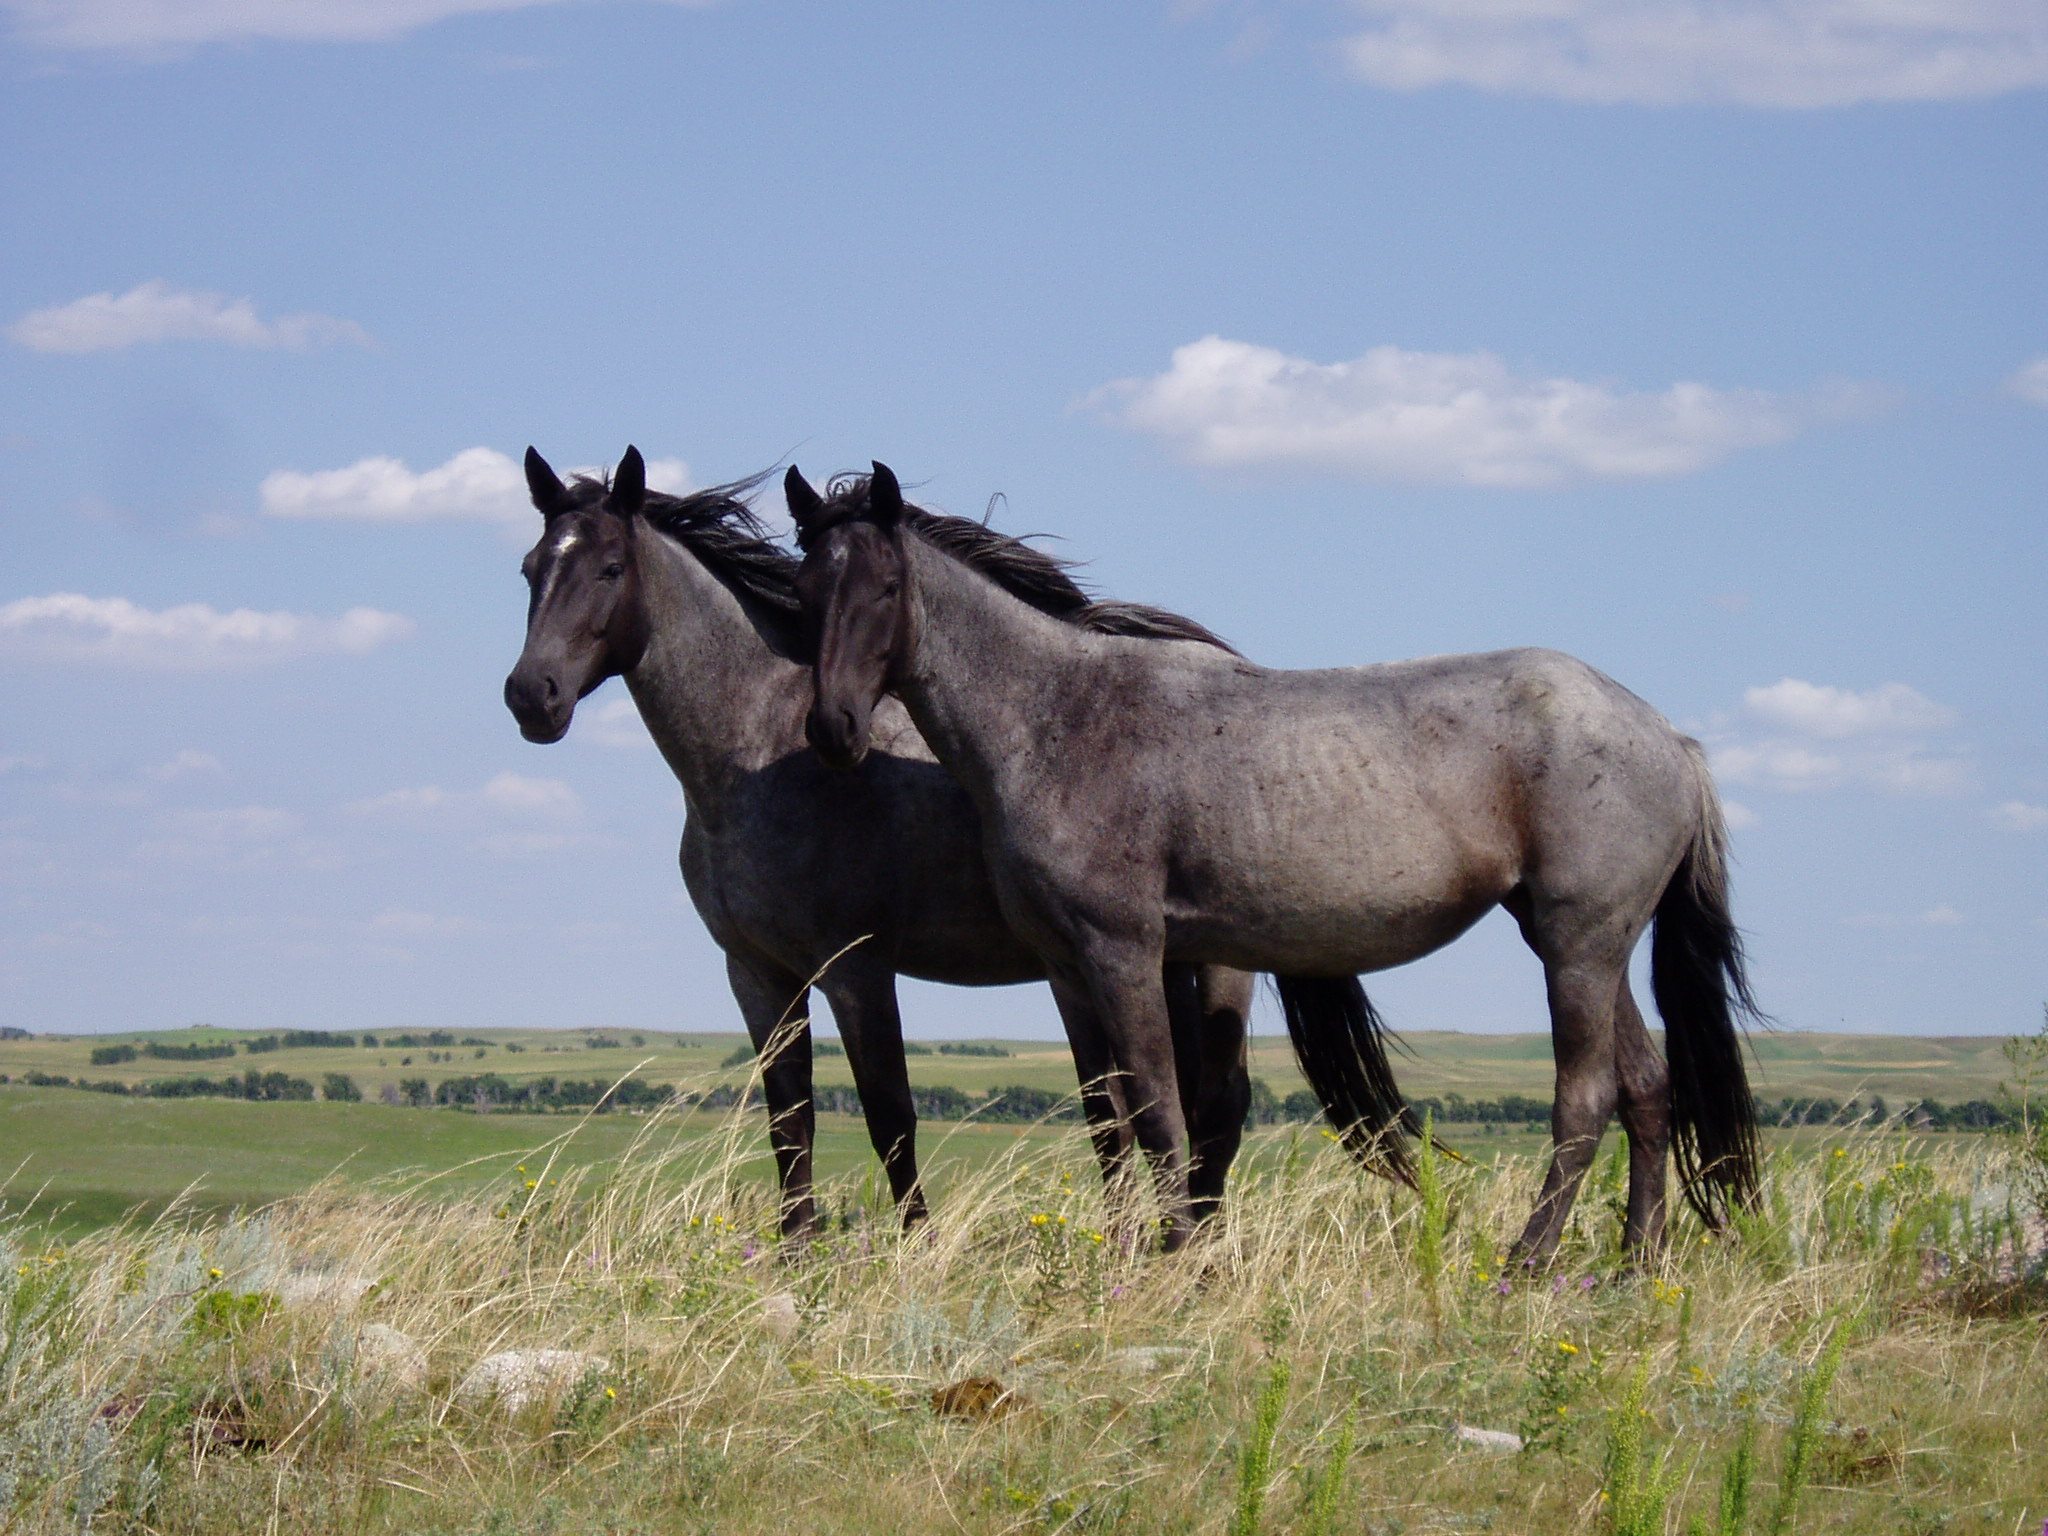
\includegraphics[height = 0.15\textheight, width = 0.4\textwidth]{horse_000005}
	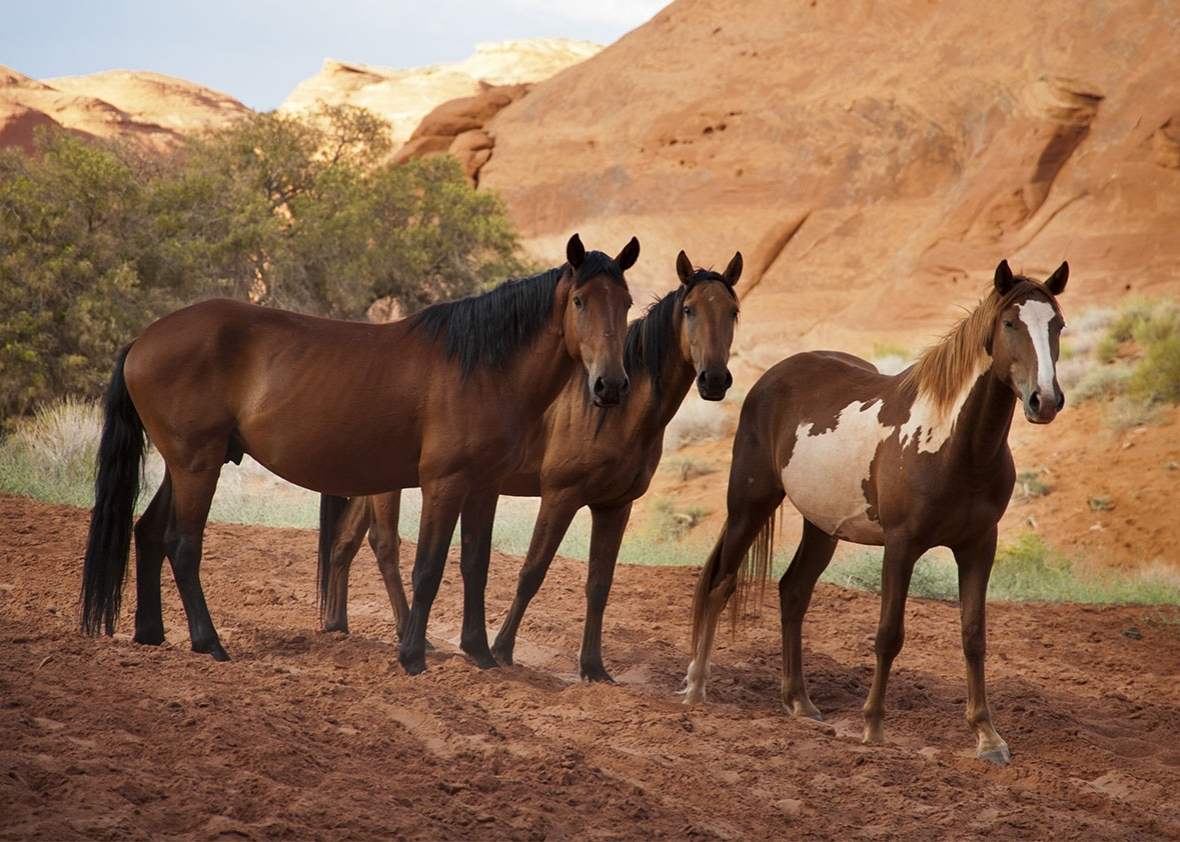
\includegraphics[height = 0.15\textheight, width = 0.4\textwidth]{horse_000006}
	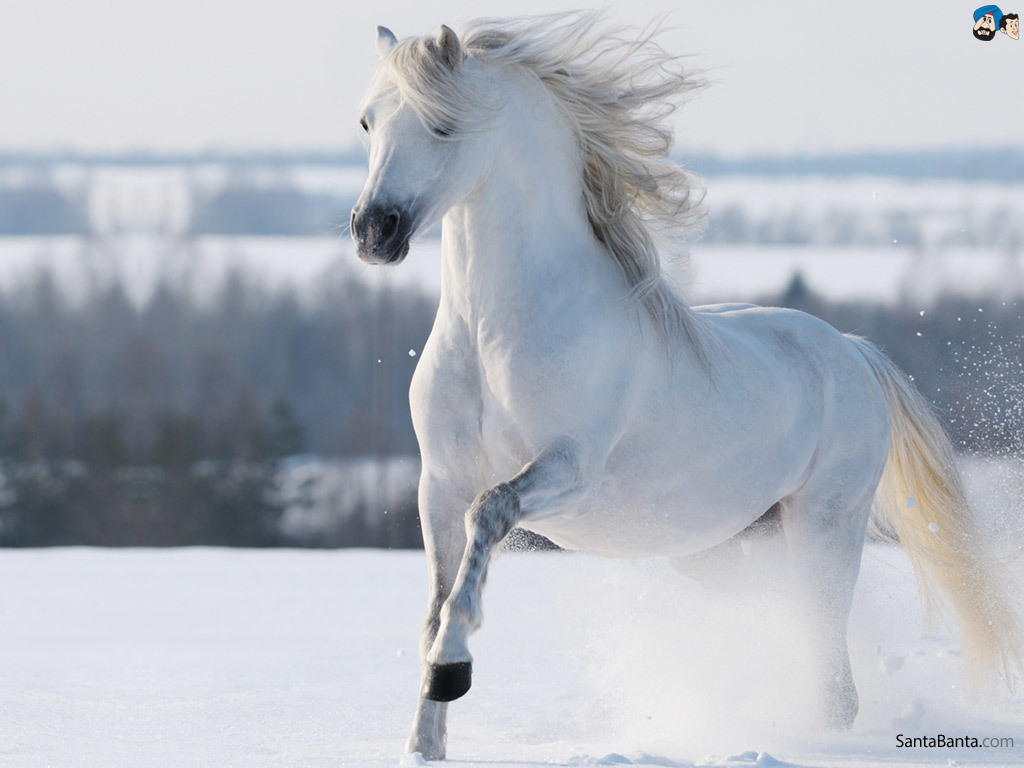
\includegraphics[height = 0.15\textheight, width = 0.4\textwidth]{horse_000007}
	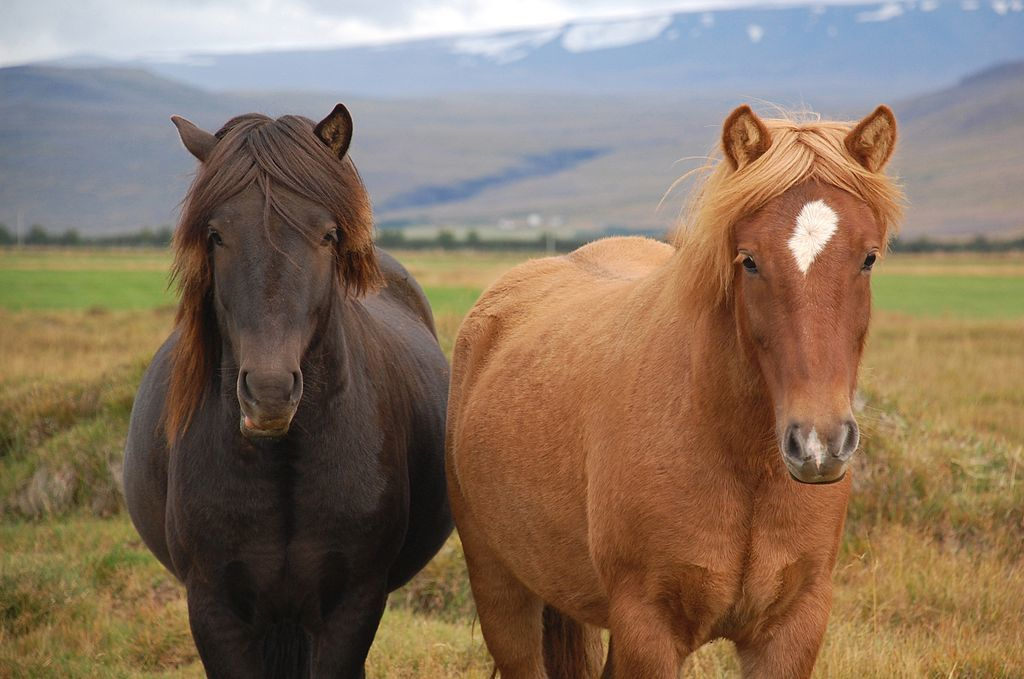
\includegraphics[height = 0.15\textheight, width = 0.4\textwidth]{horse_000008}
	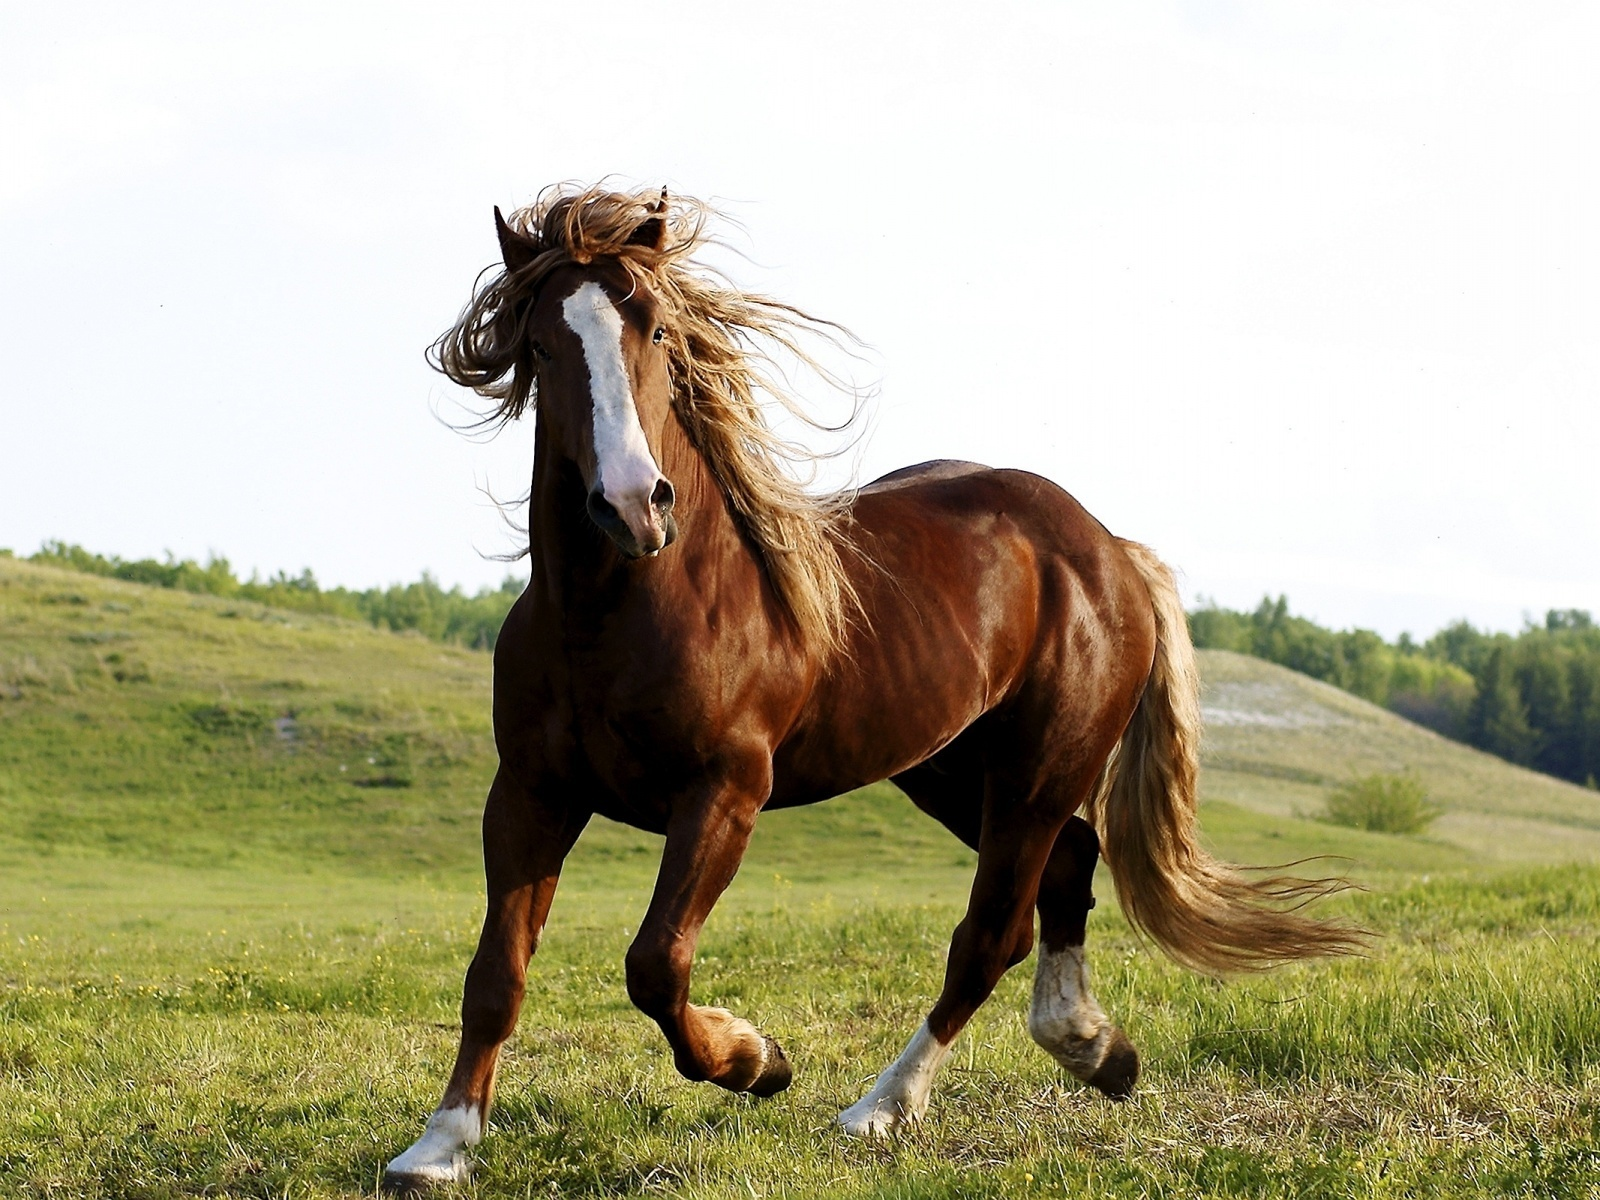
\includegraphics[height = 0.15\textheight, width = 0.4\textwidth]{horse_000009}
	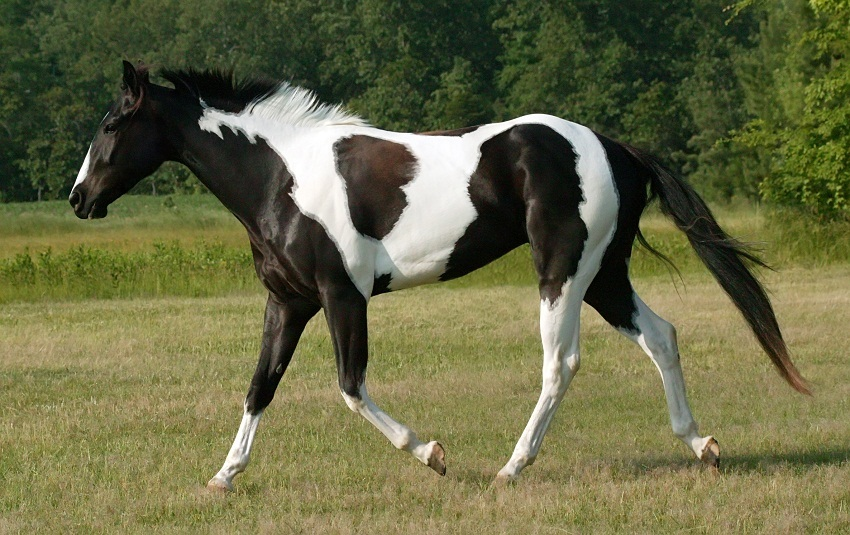
\includegraphics[height = 0.15\textheight, width = 0.4\textwidth]{horse_000010}

	\caption{Horse images used : the five first are ranked first.}
	\label{fig_2P2_1}
\end{figure}

\clearpage

\question{QP2.2: What is the best performance (measured by precision at rank-36) you were able to achieve for the horse and the car class? How many training images did you use? For each of the two classes, show examples of your training images, show the top ranked 36 images, and report the precision at rank-36. Compare the difficulty of of retrieving horses and cars.}

\begin{figure}[ht!]
	\centering
	\begin{subfigure}[b]{\textwidth}
		\centering
		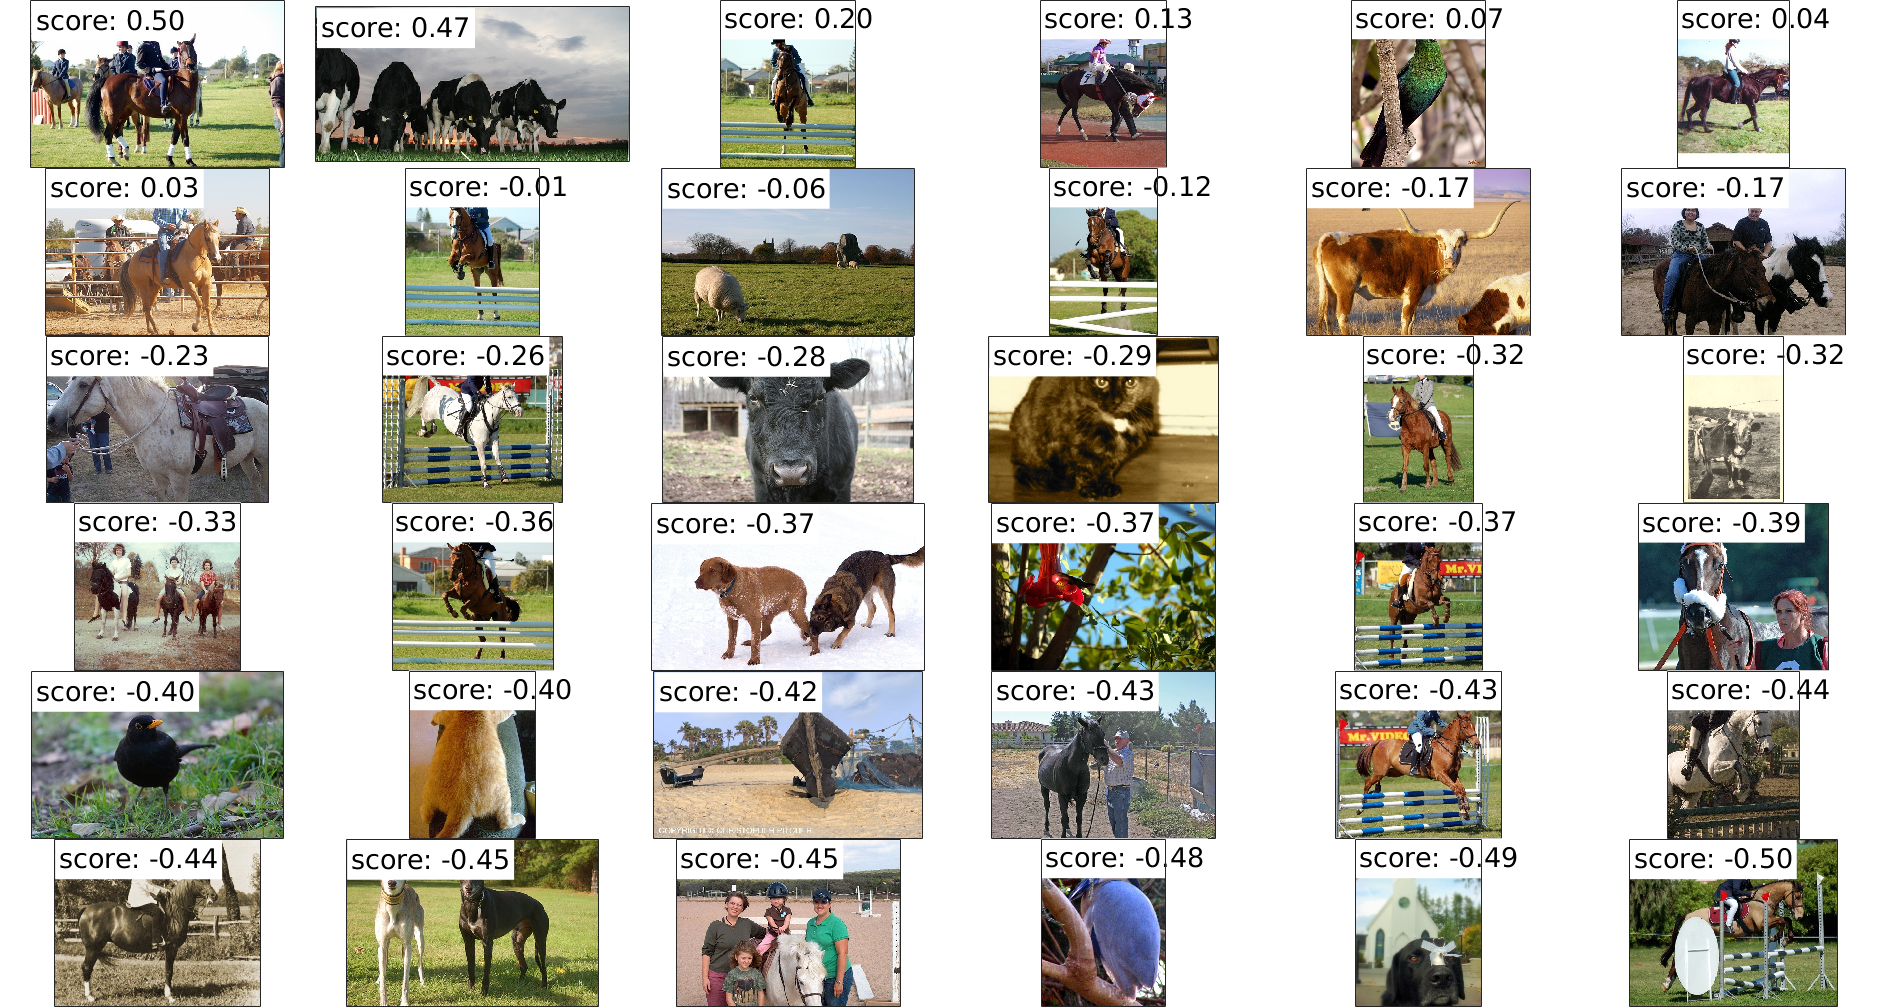
\includegraphics[width = 1.0\textwidth]{IIP22_horses_top36}
		\subcaption{Correctly retrieved in the top 36: 21 for 30 training images}
		\label{fig_IIP22_horses}
	\end{subfigure}
	\begin{subfigure}[b]{\textwidth}
		\centering
		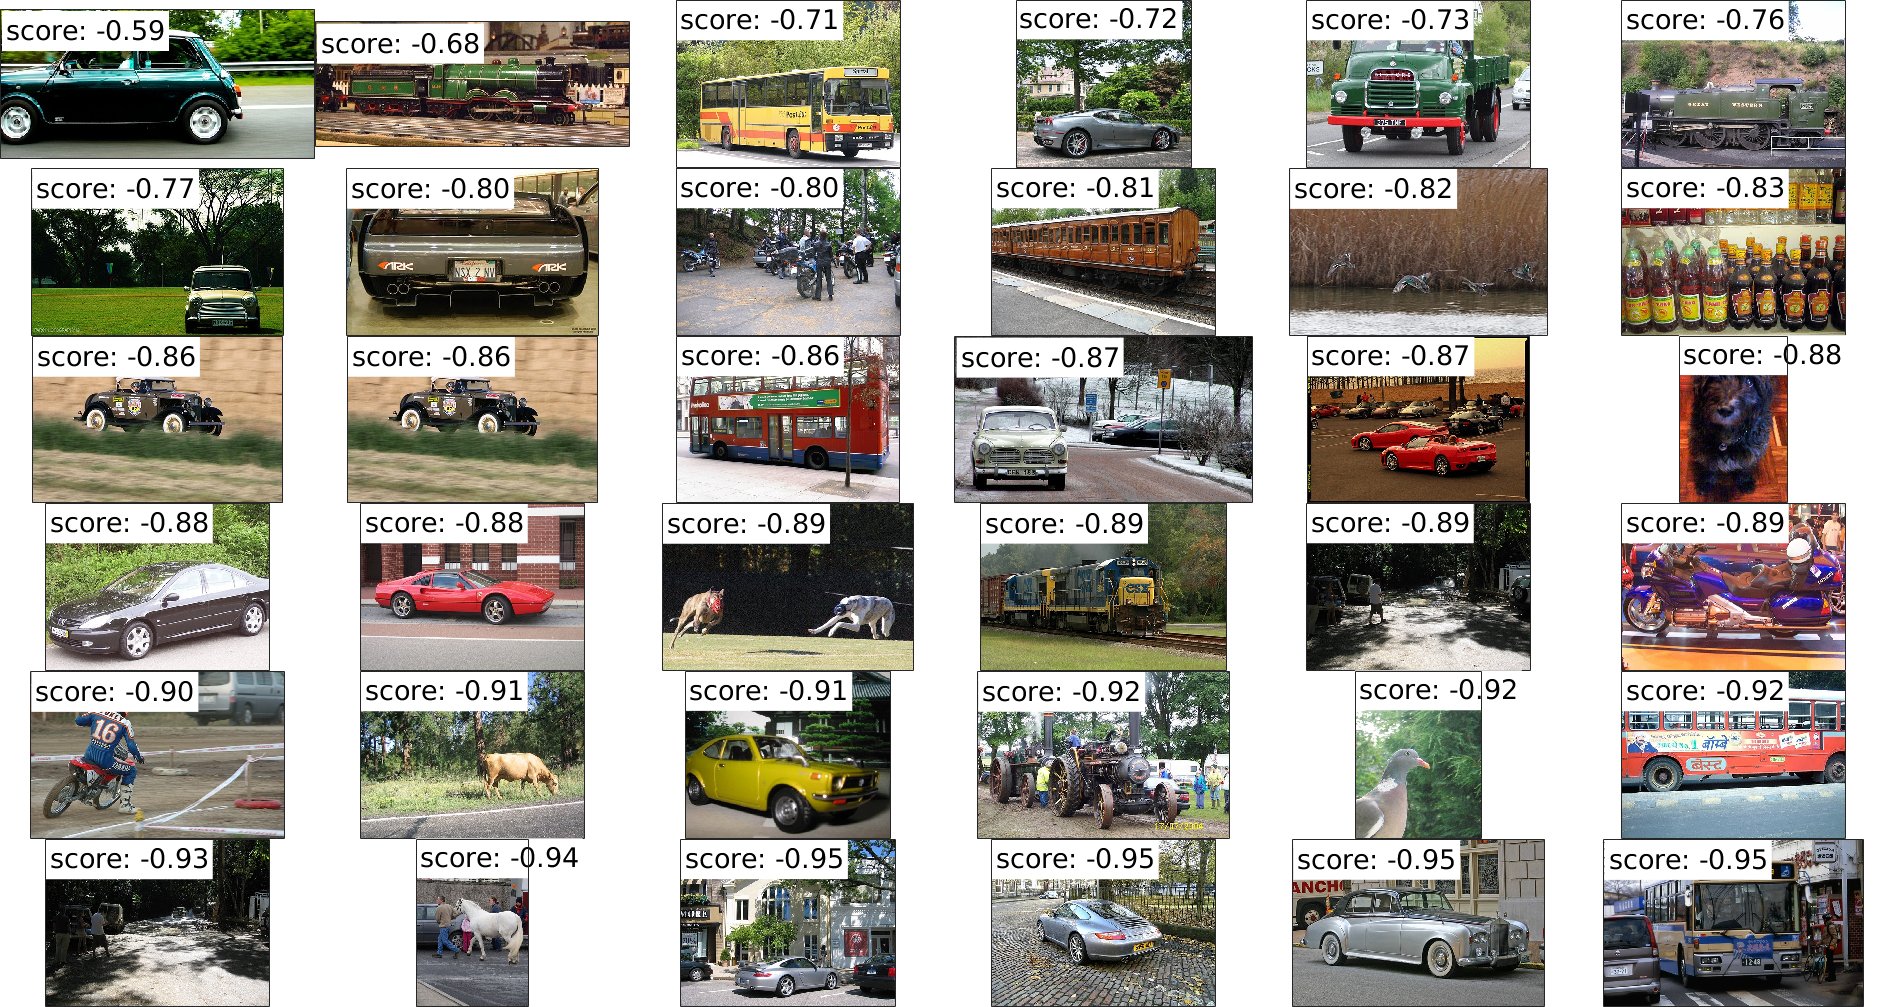
\includegraphics[width = 1.0\textwidth]{IIP22_cars_top36}
		\subcaption{Correctly retrieved in the top 36: 23 for 10 training images}
		\label{fig_IIP22_cars}
	\end{subfigure}
	\caption{Training classifier using internet image search}
	\label{fig_2P22}
\end{figure}

In figure~\ref{fig_2P22} is shown the top 36 ranking obtained after 30 training iamges for horses and 10 training image for cars. The precision at 36 is 23 for the cars class and 21 for the horses class, even with 3 times more training images, meaning it's is more difficult to retrieve horses than cars, in the test set at least.


\part{First order methods}

\question{QH1: Compare the dimension of VLAD and BoVW vectors for a given value of K. What should be the relation of the K in VLAD to the K in BoVW in order to obtain descriptors of the same dimension? You can ignore tiling.}

\question{QH2: Replace the encoding used in exercise1 with the VLAD encoding, and repeat the classification experiments for the three classes of Part I (Both linear and Hellinger kernel). How do the results compare to the BoVW encoding? Report mAP results in a table. No need to report all precision-recall curves.}

\begin{table}[ht!]
	\centering
	\begin{tabular}{|l | p{3.5cm} | p{3.5cm}|}
		\hline
		Class      & AP in test Hellinger Kernel, BoVW & AP in test Hellinger Kernel, VLAD & AP in test linear Kernel, VLAD \\\hline\hline
		Aeroplanes & \(70.72~\%\)                      & \(74.62~\%\) & \(70.72~\%\)                     \\\hline
		Motorbikes & \(63.25~\%\)                      & \(68.82~\%\)                      \\\hline
		Persons    & \(77.39~\%\)                      & \(\75.54~\%\)                     \\\hline
	\end{tabular}
	\caption{Effect of using VLAD descriptor instead of BoVW descriptor}
	\label{tab_III2}
\end{table}



\end{document}
